\documentclass[pdf]{beamer}\usepackage[]{graphicx}\usepackage[]{color}
%% maxwidth is the original width if it is less than linewidth
%% otherwise use linewidth (to make sure the graphics do not exceed the margin)
\makeatletter
\def\maxwidth{ %
  \ifdim\Gin@nat@width>\linewidth
    \linewidth
  \else
    \Gin@nat@width
  \fi
}
\makeatother

\definecolor{fgcolor}{rgb}{0.345, 0.345, 0.345}
\newcommand{\hlnum}[1]{\textcolor[rgb]{0.686,0.059,0.569}{#1}}%
\newcommand{\hlstr}[1]{\textcolor[rgb]{0.192,0.494,0.8}{#1}}%
\newcommand{\hlcom}[1]{\textcolor[rgb]{0.678,0.584,0.686}{\textit{#1}}}%
\newcommand{\hlopt}[1]{\textcolor[rgb]{0,0,0}{#1}}%
\newcommand{\hlstd}[1]{\textcolor[rgb]{0.345,0.345,0.345}{#1}}%
\newcommand{\hlkwa}[1]{\textcolor[rgb]{0.161,0.373,0.58}{\textbf{#1}}}%
\newcommand{\hlkwb}[1]{\textcolor[rgb]{0.69,0.353,0.396}{#1}}%
\newcommand{\hlkwc}[1]{\textcolor[rgb]{0.333,0.667,0.333}{#1}}%
\newcommand{\hlkwd}[1]{\textcolor[rgb]{0.737,0.353,0.396}{\textbf{#1}}}%
\let\hlipl\hlkwb

\usepackage{framed}
\makeatletter
\newenvironment{kframe}{%
 \def\at@end@of@kframe{}%
 \ifinner\ifhmode%
  \def\at@end@of@kframe{\end{minipage}}%
  \begin{minipage}{\columnwidth}%
 \fi\fi%
 \def\FrameCommand##1{\hskip\@totalleftmargin \hskip-\fboxsep
 \colorbox{shadecolor}{##1}\hskip-\fboxsep
     % There is no \\@totalrightmargin, so:
     \hskip-\linewidth \hskip-\@totalleftmargin \hskip\columnwidth}%
 \MakeFramed {\advance\hsize-\width
   \@totalleftmargin\z@ \linewidth\hsize
   \@setminipage}}%
 {\par\unskip\endMakeFramed%
 \at@end@of@kframe}
\makeatother

\definecolor{shadecolor}{rgb}{.97, .97, .97}
\definecolor{messagecolor}{rgb}{0, 0, 0}
\definecolor{warningcolor}{rgb}{1, 0, 1}
\definecolor{errorcolor}{rgb}{1, 0, 0}
\newenvironment{knitrout}{}{} % an empty environment to be redefined in TeX

\usepackage{alltt}
\mode<presentation>
\usetheme[compress]{Singapore} %Berkeley, Palo Alto, Singapore, Warsaw
%\usetheme[compress]{Berlin} 
%\usetheme[compress]{Madrid} 
%\usecolortheme{seagull}  %Beaver, dolphin, dove, lily, orchid, seagull, seahorse

%\usefonttheme{serif}
% font themes: default, professionalfonts, serif, structurebold, structureitalicserif, structuresmallcapsserif

\usepackage{graphicx}
\usepackage{pgf}
\usepackage{array}
\usepackage{tabularx}
\usepackage{booktabs}          %% Used in risk tables
\usepackage{multirow}          %% Used in decision tables
\usepackage{multicol}          %% Used in the toc
\usepackage[T1]{fontenc}  %to use < or > in tables

%\graphicspath{C:/Users/Chantel.Wetzel/Documents/GitHub/POP_2017}
\newcolumntype{Y}{>{\centering\arraybackslash}X}
\newcommand{\specialcell}[2][c]{\begin{tabular}[#1]{@{}c@{}}#2\end{tabular}}
\newcommand{\subscr}[1]{$_{\text{#1}}$}
\newcommand{\Fforty}{F_{\text{SPR}=40\%}}       % Needs to be done as $\Fforty$
\newcommand{\Bforty}{B_{\text{SPR}=40\%}}

\setbeamersize{text margin left=0.1in}
\setbeamersize{text margin right=0.1in}

\definecolor{pageCol}{rgb}{0.5,0.5,1.0}

\usepackage{tikz}

\usebackgroundtemplate{
  \tikz[overlay,remember picture] 
  \node[opacity=0.3, at=(current page.south east),anchor=south east,inner sep=0pt] {
    
\includegraphics[height=0.5in]{noaalogo.jpg}};
}

\setbeamertemplate{footline}
{
  \begin{beamercolorbox}[wd=.05\paperwidth,ht=0ex,dp=0ex,left]{framenumber in head/foot}%
    \insertframenumber/\inserttotalframenumber
    
  \end{beamercolorbox}%
}
\setbeamercolor{footline}{fg=pageCol}

\newcounter{saveenumi}

%<<load_everything, echo = FALSE, message=FALSE, results='hide', warning=FALSE>>=
%     source("C:/Users/Chantel.Wetzel/Documents/GitHub/POP_2017/Presentation/0_Run_Model_Presentation.R")
%      #create.plots = TRUE
%      #Run.Model.Present(create.plots)
%     source("C:/Users/Chantel.Wetzel/Documents/GitHub/POP_2017/Presentation/tables/catch.R")
%@

%<<load_mod1, echo = FALSE, message=FALSE, results='hide', warning=FALSE>>=
%  load("C:/Users/Chantel.Wetzel/Documents/GitHub/POP_2017/Presentation/SS_output.RData")
%@

\newcommand{\mytableofcontents}{
  \begin{frame}[t]
  \frametitle{Outline}
  %\begin{multicols}{2}
  \tableofcontents[
    currentsection, sectionstyle=show/show, subsectionstyle=show/show/hide,
  ]
  %\end{multicols}
  \end{frame}
}
\AtBeginSection[]{\mytableofcontents}

%------------------------------------------------------------------------------------
% Title Page
%------------------------------------------------------------------------------------
\title{Petrale sole 2019 Assessment}
\subtitle{Updated Data and Results}
\author{Chantel Wetzel$^{1}$}
\institute[NWFSC]{
Northwest Fisheries Science Center$^1$ \\
\medskip
}
\date{{\footnotesize SSC Review \\ August 20, 2019}}
\IfFileExists{upquote.sty}{\usepackage{upquote}}{}
\begin{document}

\begin{frame}
  \titlepage
\end{frame}


%------------------------------------------------------------------------------------
\section{Model Summary}
%------------------------------------------------------------------------------------
\subsection{Overview}
\begin{frame}{Petrale sole (\textit{Eopsetta jordani})}
\begin{columns}
  \begin{column}{0.5\textwidth}
      \begin{itemize}
        \item Distributed from  Alaska Aleutian Islands to Northern California
        \item Typically distributed between 200 - 400 meters during summer months
        \item Semi-demersal and can be pelagic
        \item Both sexes move to deeper water with age
        \item Currently, no evidence for genetic differences in the assessment area
      \end{itemize}
  \end{column}
  
  \begin{column}{0.5\textwidth}
    %\includegraphics[scale = 0.25]{C:/Users/Chantel.Wetzel/Documents/GitHub/POP_2017/Sebastes_alutus.png}
    \begin{itemize}
        \item Females move to deeper waters post-spawning during winter months and return inshore in spring.
      \end{itemize}
  \end{column}
\end{columns}
\end{frame}


\subsection{Landings}
\begin{frame}{Landings}
  \begin{center}
    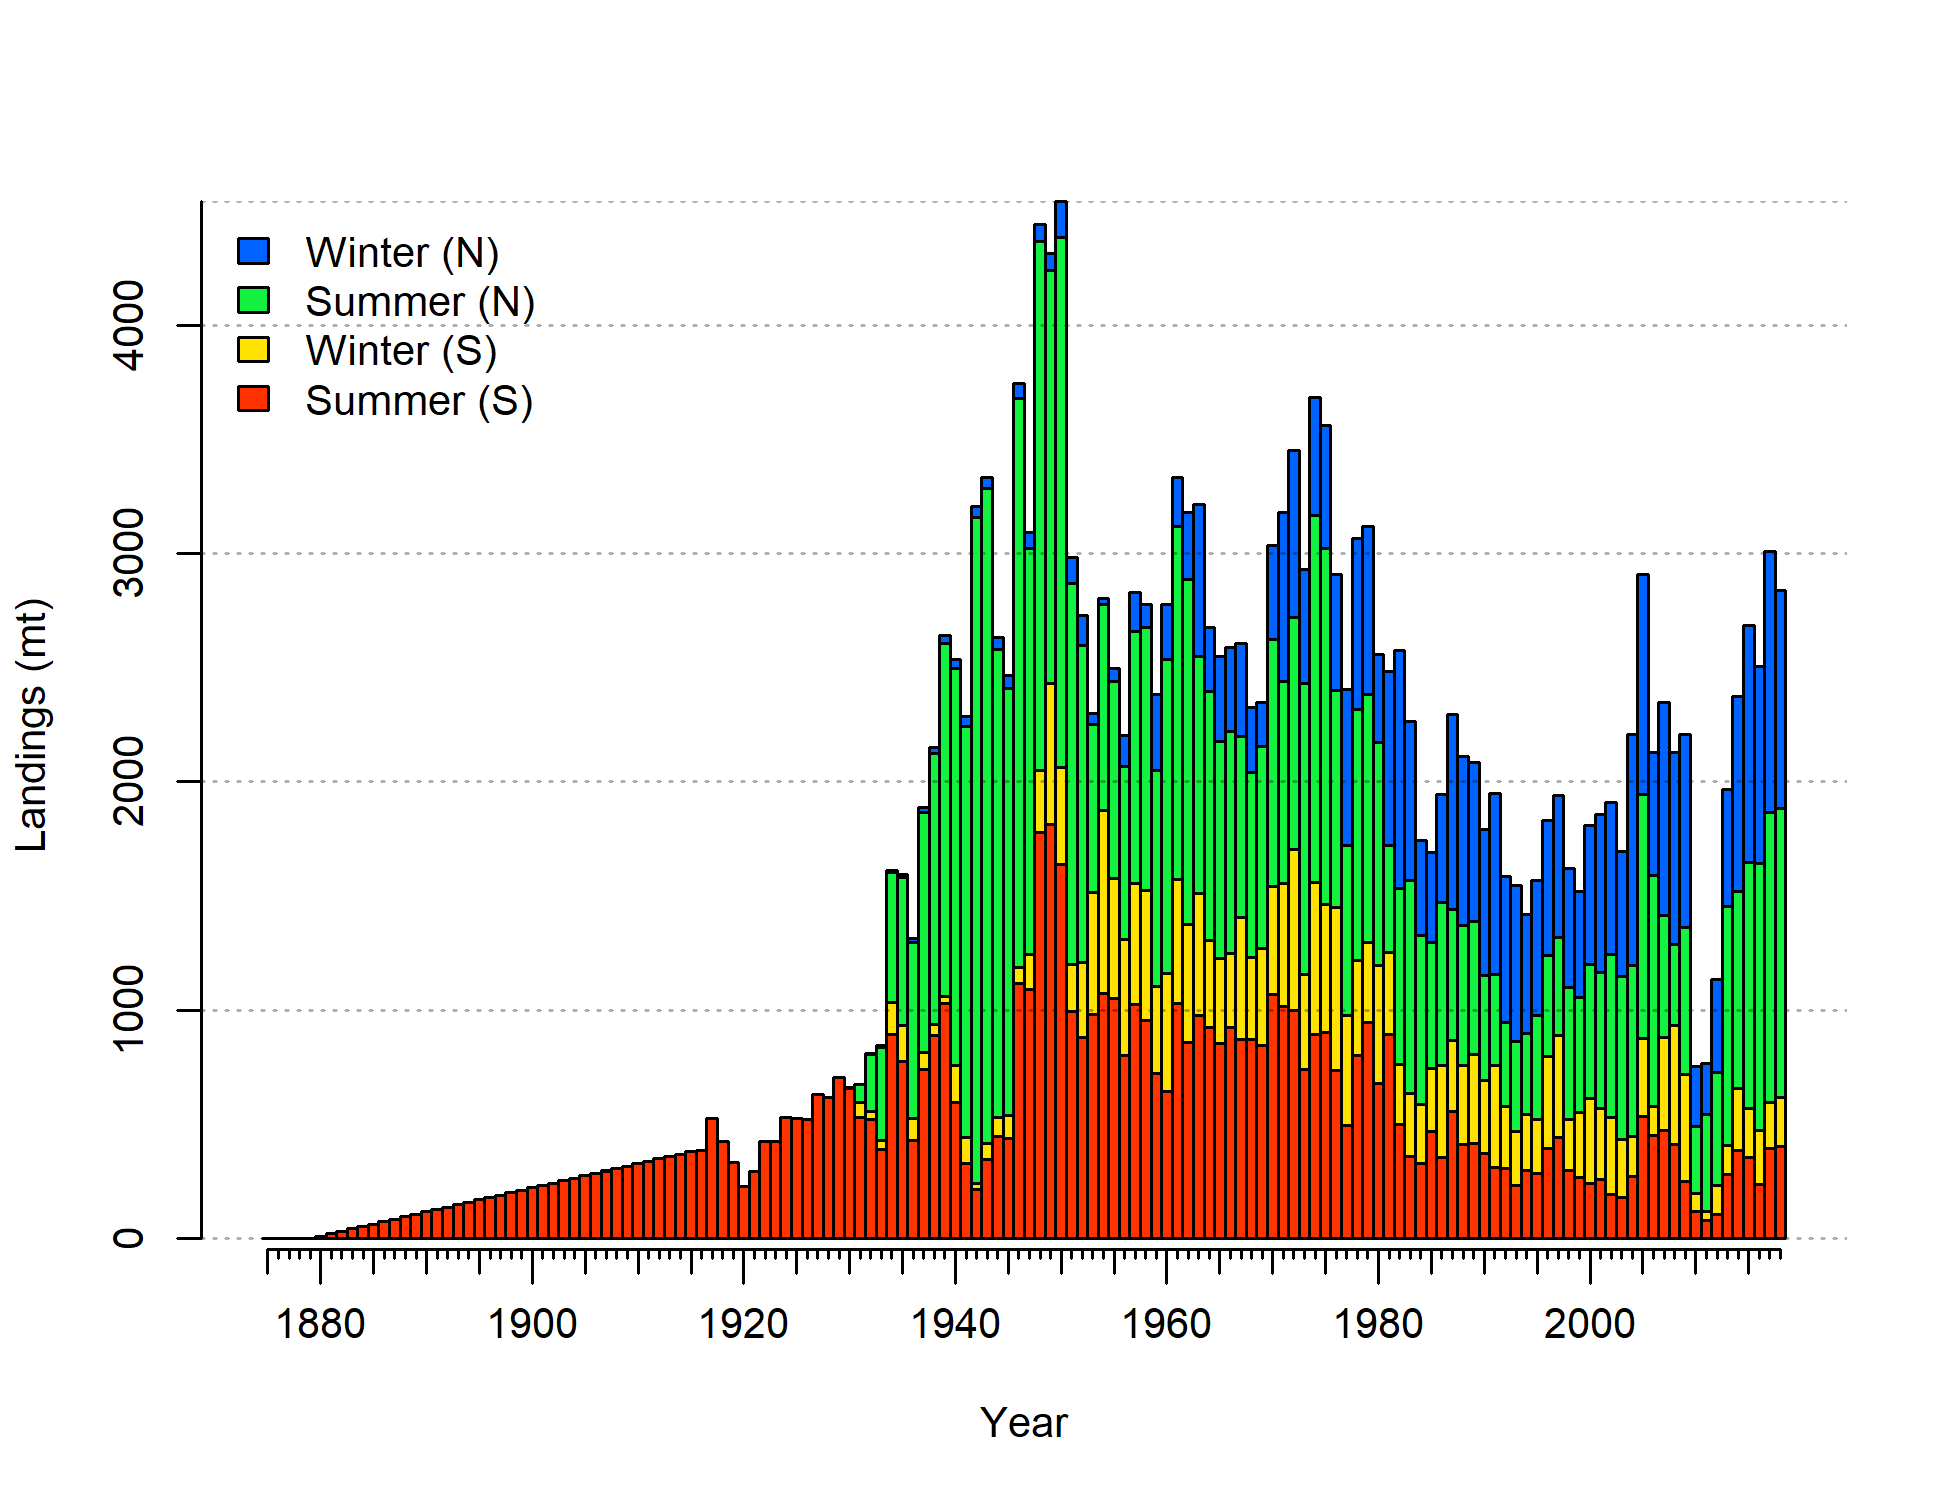
\includegraphics[scale = 0.40]{r4ss/catch2 landings stacked.png}
  \end{center}
\end{frame}



\begin{frame}{Landings & Removals Over the Last 10-Years}
  \begin{table}[ht]
  \centering
  \begin{tabular}{p{0.5in}p{0.5in}p{0.5in}p{0.5in}p{0.5in}p{0.5in}p{0.5in}}
  Year & Winter-N & Summer-N & Winter-S & Summer-S & Total Landings & Total Removals \\ 
  \hline
  2009 & 874  & 642  & 470 & 250 & 2209 & 2344\\ 
  2010 & 264  & 292  & 78  & 121 & 755  & 869 \\ 
  2011 & 224  & 427  & 40  & 78  & 768  & 785 \\ 
  2012 & 410  & 497  & 124 & 108 & 1135 & 1153\\ 
  2013 & 513  & 1045 & 130 & 280 & 1967 & 1995\\ 
  2014 & 853  & 861  & 273 & 386 & 2373 & 2392\\ 
  2015 & 1040 & 1077 & 215 & 354 & 2686 & 2704\\ 
  2016 & 865  & 1168 & 237 & 235 & 2506 & 2523\\ 
  2017 & 1142 & 1271 & 201 & 393 & 3008 & 3026\\ 
  2018 & 957  & 1262 & 218 & 402 & 2840 & 2857\\ 
  \hline
  \end{tabular}
  \end{table}
\end{frame}

\begin{frame}{Correction for the Post-STAR Model}
  \begin{itemize}
    \item Addition to California historical landings
      \begin{itemize}
        \item 1948-1968 corrections totaling 10 mt 
      \end{itemize}
    \item Survey catch removal correction
      \begin{itemize}
        \item Stock Synthesis was not removing catches for survey fleets
      \end{itemize}
    \item Weight-at-length
      \begin{itemize}
        \item Small correction to the weight-at-length values for females and males
      \end{itemize}    
  \end{itemize}
\end{frame}






\begin{frame}{Estimated Annual Recruitment}
  \begin{center}
    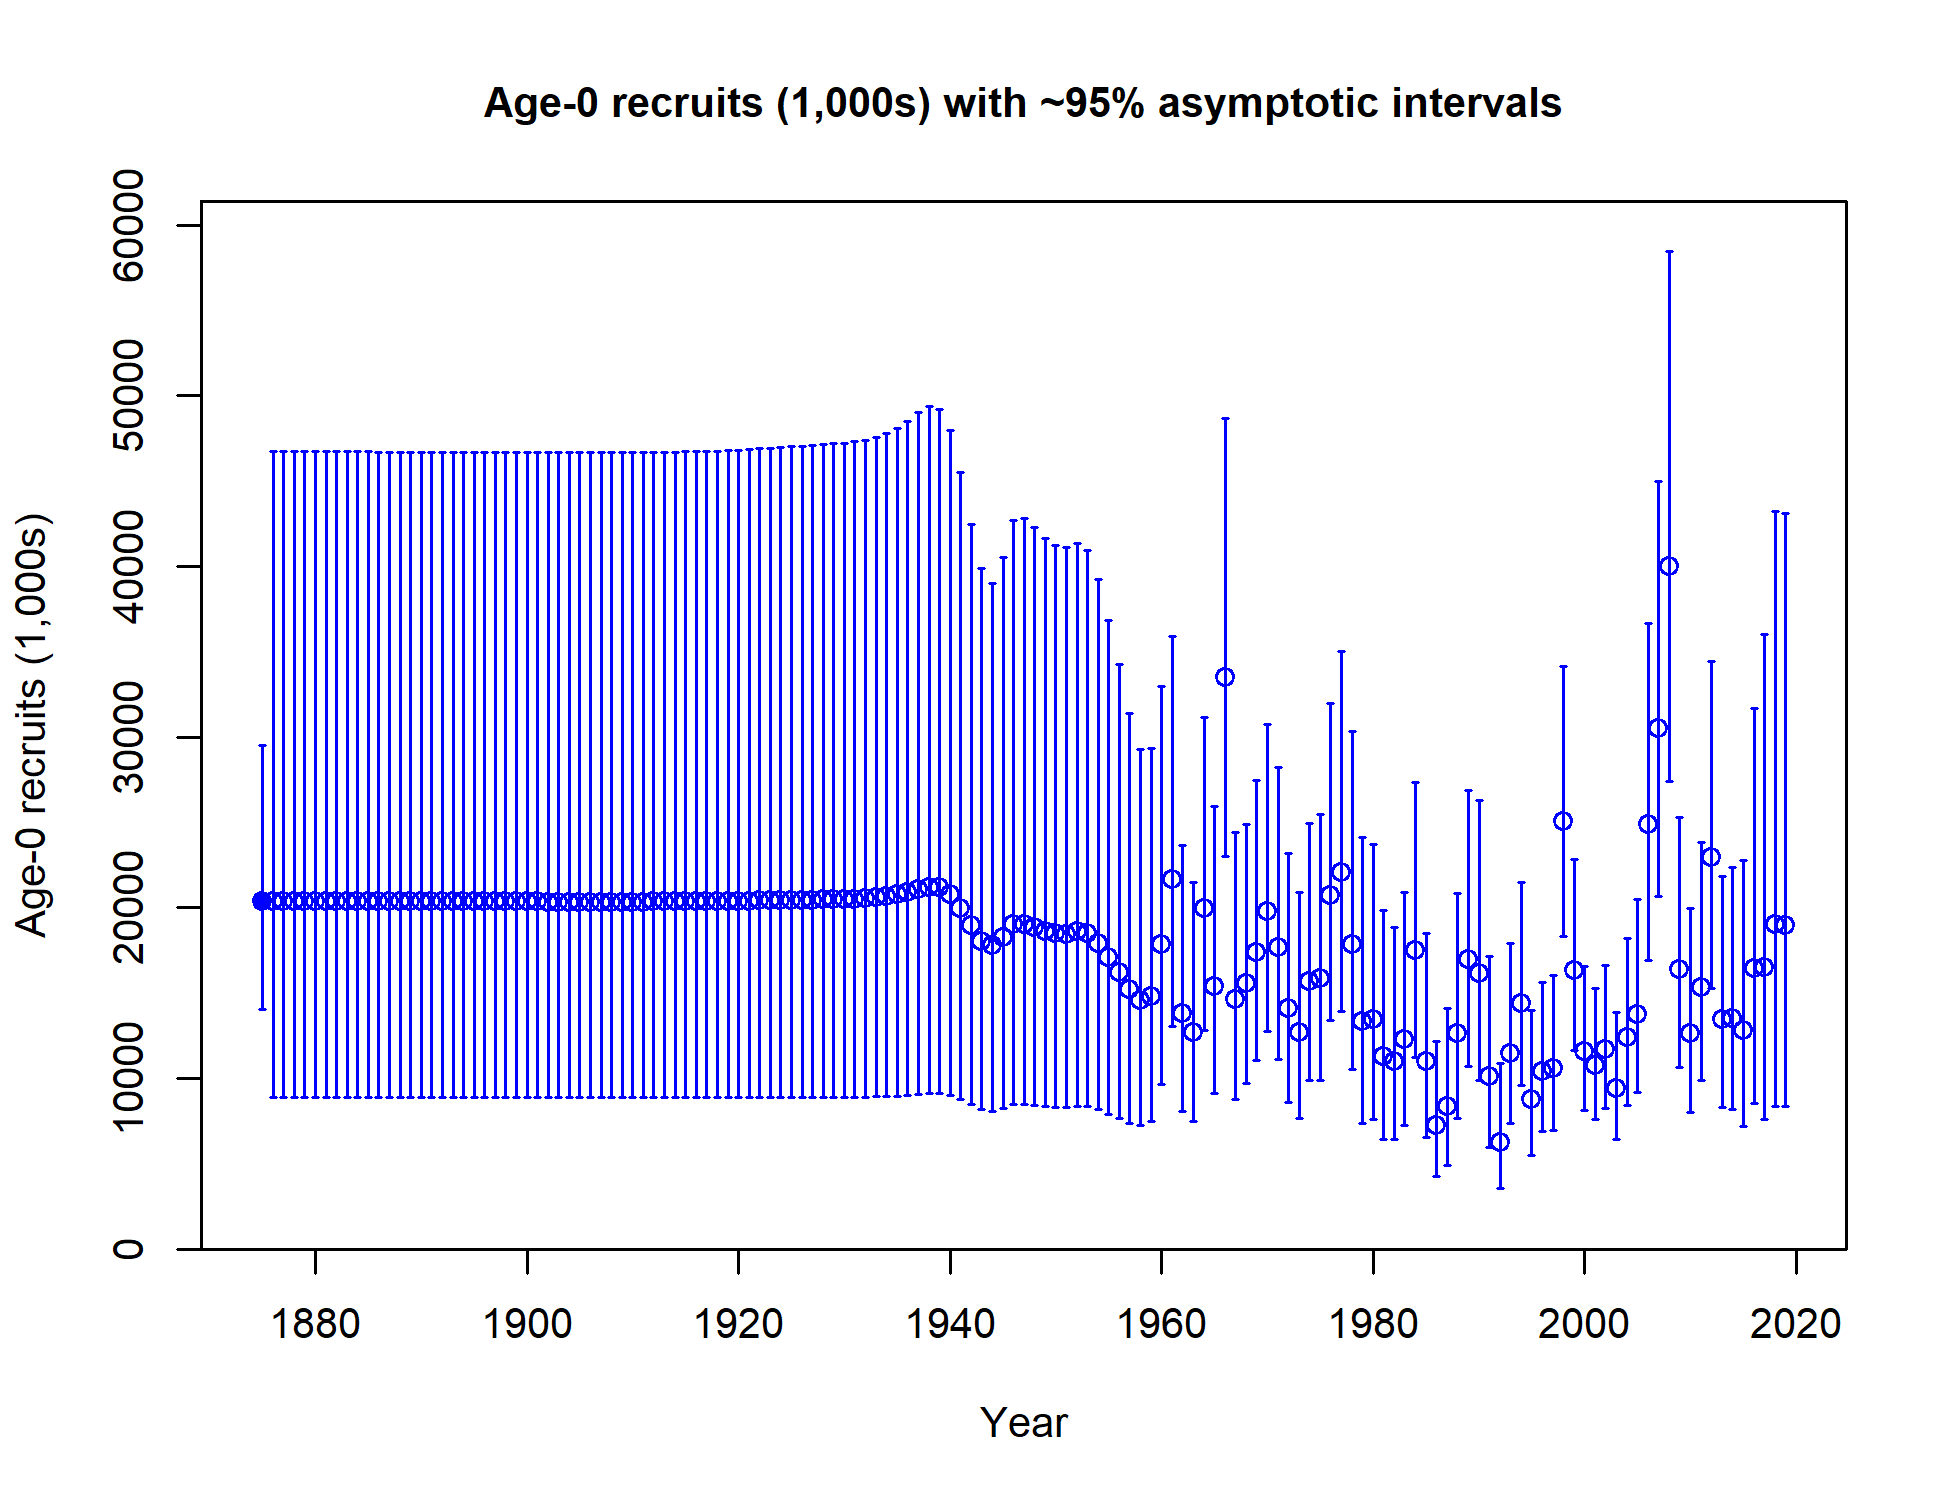
\includegraphics[scale = 0.50, trim={0cm 0cm 0cm 1.7cm}, clip]{r4ss/ts11_Age-0_recruits_(1000s)_with_95_asymptotic_intervals.png}
  \end{center}
  \begin{tikzpicture}[remember picture, overlay, shift = {(current page.center)}]
    \node[black] at (2.5, 0.75) {\tiny 2008};
    \node[black] at (3.25, -0.25) {\tiny 2013};
    \node[black] at (2.2, -0.75) {\tiny 1999 \& 2000};
  \end{tikzpicture}
\end{frame}

\begin{frame}{Estimated Annual Recruitment Deviations}
  \begin{center}
    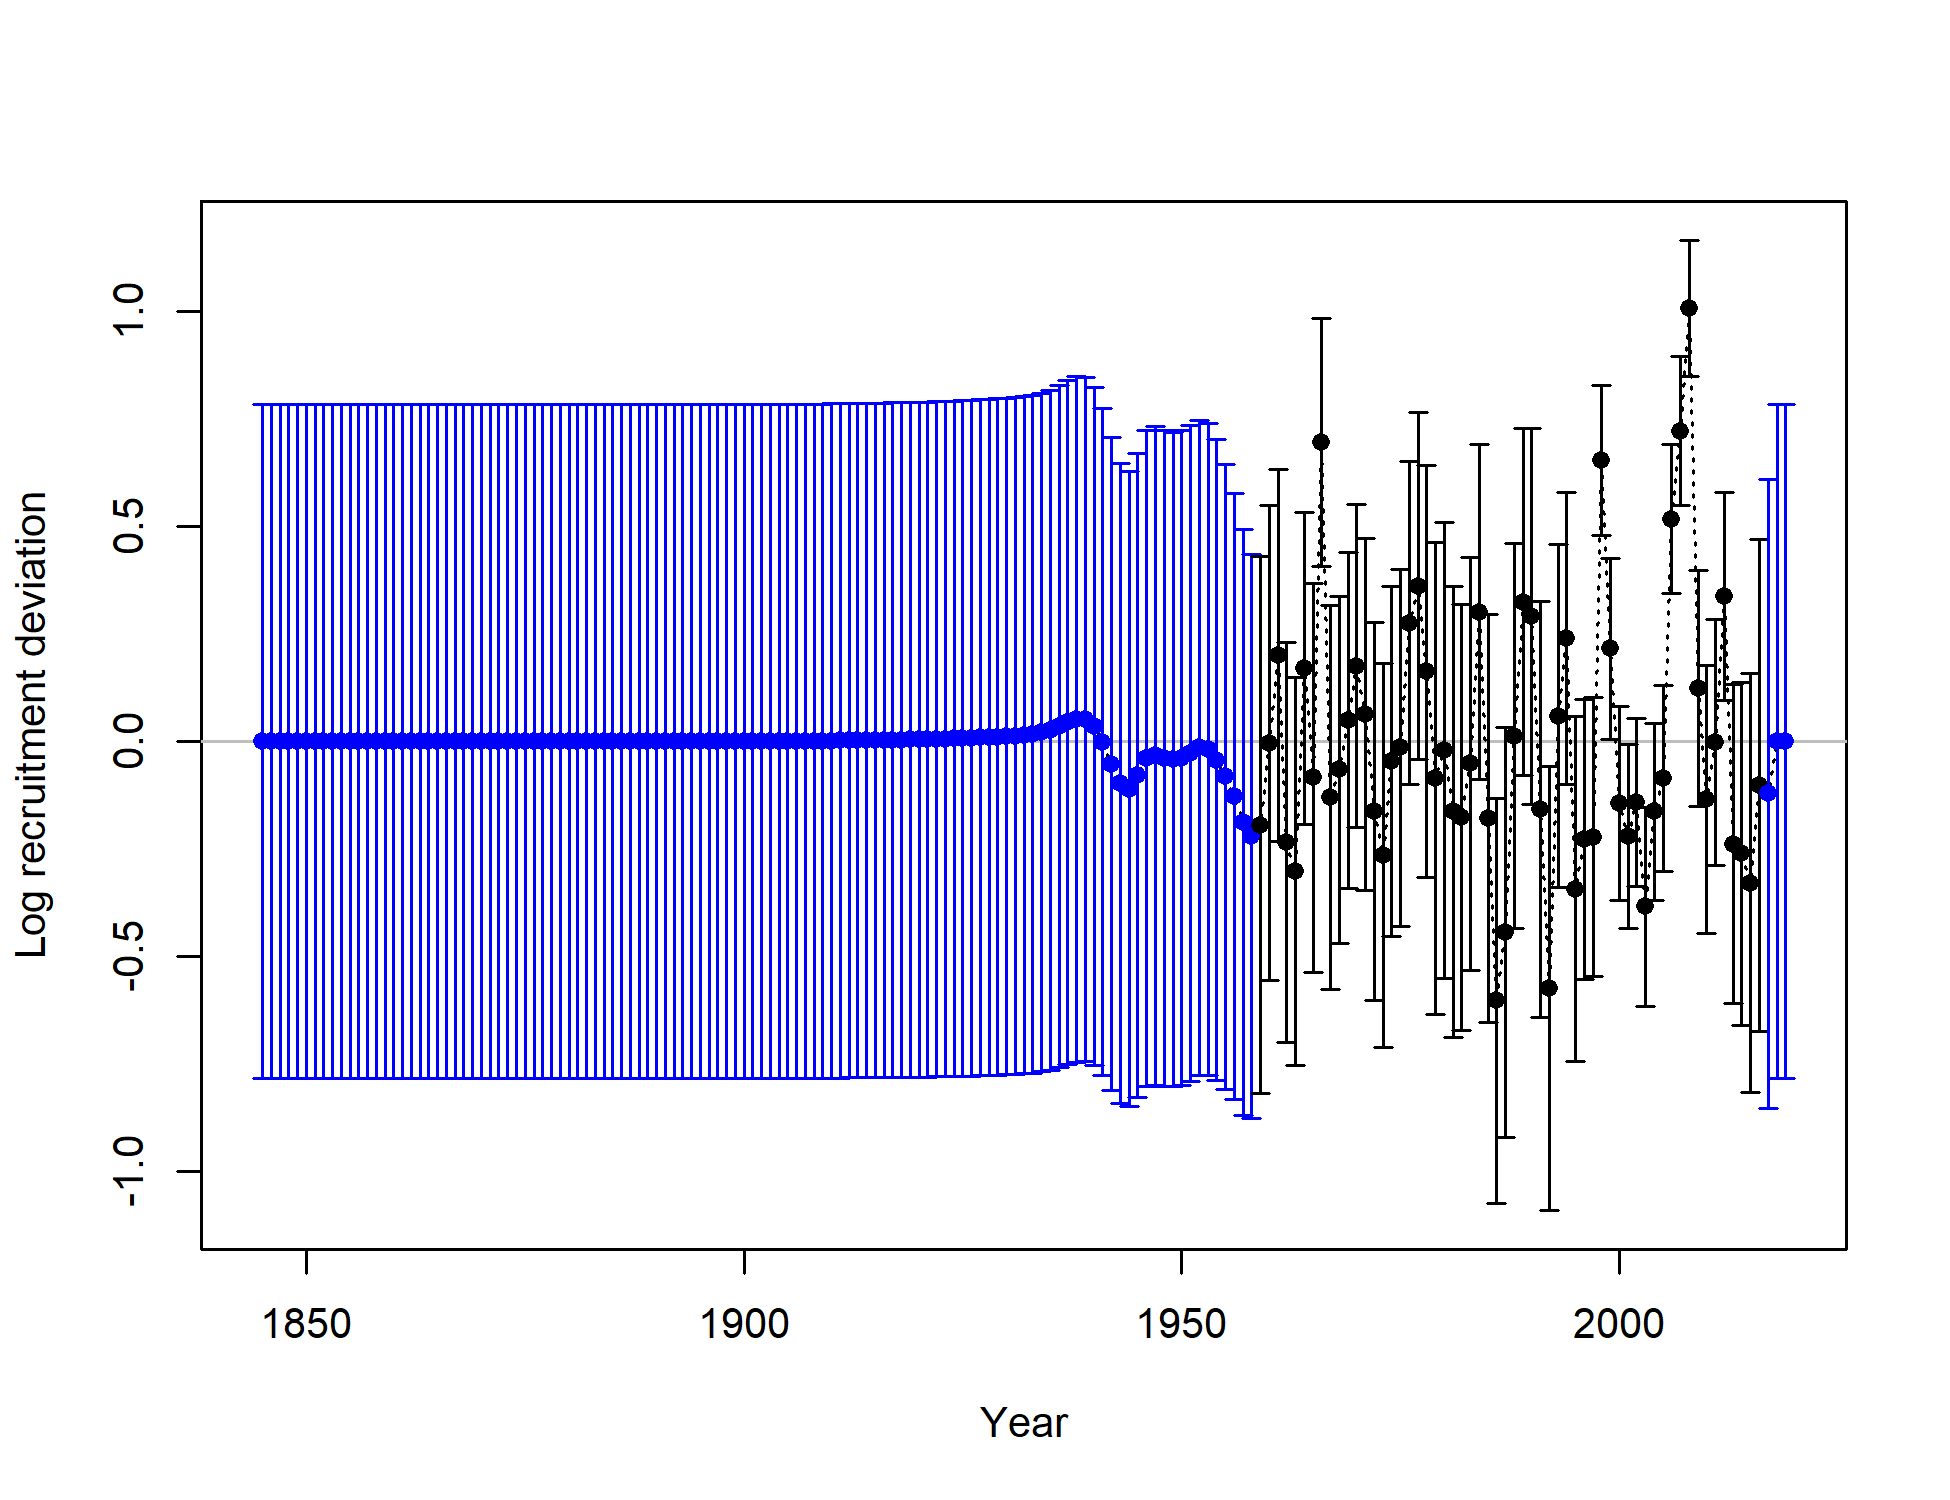
\includegraphics[scale = 0.50, trim={0cm 0cm 0cm 1.7cm}, clip]{r4ss/recdevs2_withbars.png}
  \end{center}
\end{frame}



\begin{frame}{Comparison between 2011 and 2017}
  \begin{center}
    %\includegraphics[scale = 0.50]{figures/2011_2017_Bratio.png}
  \end{center}
\end{frame}

\begin{frame}{Major Changes Between the Previous and Current Assessment}
  \begin{itemize}
    \item Steepness 
      \begin{itemize}
        \item The 2011 assessment fixed $h$ = 0.40
        \item The current assessment fixed $h$ = 0.50 
      \end{itemize}
    \item Natural Mortality
      \begin{itemize}
        \item The 2011 assessment fixed $M$ = 0.05 for females, males estimated $M$ = 0.051
        \item The current assessment fixed $M$ = 0.054 for both sexes
      \end{itemize}
    \item Landings History
    \item Maturity and Fecundity
    \item Fleet and Survey Selectivities 
      %\begin{itemize}
      %  \item Fishery and survey specific estimated in current assessment 
        %- 60.6\% fixed 73.1\% estimated
      %\end{itemize}
  \end{itemize}
\end{frame}

\begin{frame}{2011 Model Data "Update"}
  \begin{itemize}
    %\item Added layers of new data cumulatively while retaining 2011 modeling assumptions
  \end{itemize}
  \begin{center}
    %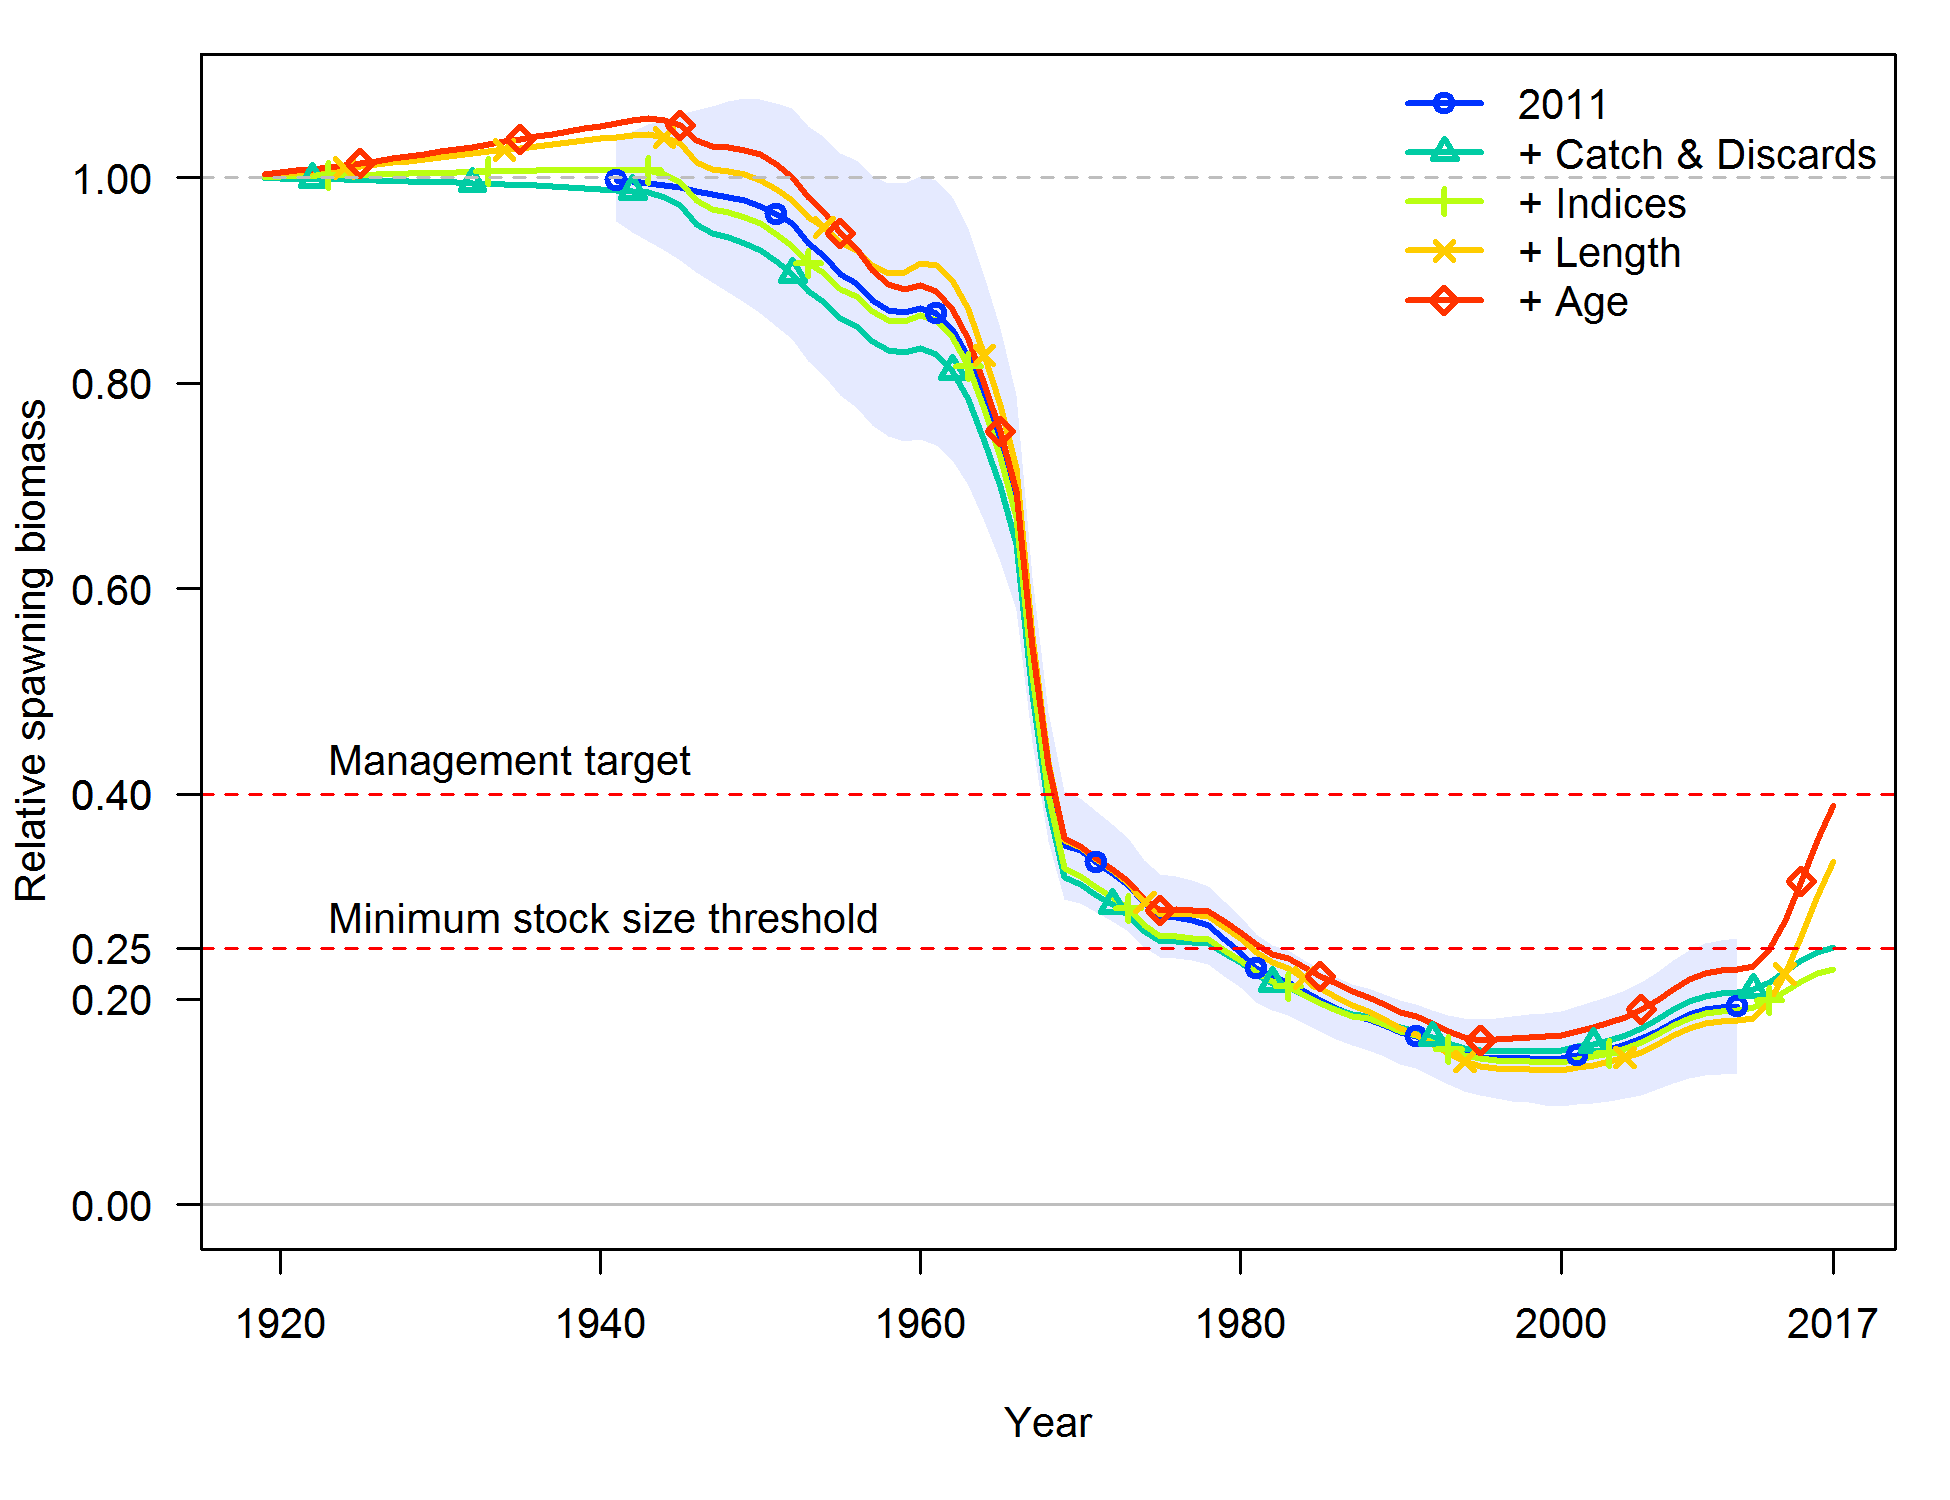
\includegraphics[scale = 0.42]{figures/Data_Bratio_uncertainty.png}
  \end{center}
\end{frame}

\begin{frame}{2017 Base Model Sensitivities}
  %\begin{center}
    %\includegraphics[scale = 0.28]{figures/SSB_sensitivities_1.png}
    %\includegraphics[scale = 0.28]{figures/Bratio_sensitivites_1.png}
  %\end{center}
\end{frame}


\subsection{Uncertainties}
\begin{frame}{Key Sources of Uncertainty}
  \begin{itemize}
    \item Steepness
    \begin{itemize}
      \item Fixed at 0.50 within the base model.  Likelihood profile over steepness indicates no information in data concerning steepness.  Fixing the value at the steepness prior value of 0.72 results in stock status 97\% of unfished.
    \end{itemize}
    \item Natural Mortality
      \begin{itemize}
        \item Fixed at 0.054 for males and females, the mean of the prior when maximum age is 100.  Likelihood profile relatively flat around the prior.
      \end{itemize}
    \item Recruitment 
      \begin{itemize} 
        \item Estimated large recruitments in 2008 and 2013. 
        \item Setting these recruitments equal to the stock-recruitment curve results in a decline in stock status to ~54\%.
      \end{itemize}
    \item{NWFSC shelf-slope age data}
      \begin{itemize}
        \item Treating these data as either conditional age-at-length or as marginals results in differing estimates of $R_0$ and final stock status.
      \end{itemize}
  \end{itemize}
\end{frame}


%------------------------------------------------------------------------------------
\section{Biology}

%------------------------------------------------------------------------------------

\subsection{Fecundity}
\begin{frame}{Fecundity}
  \begin{center}
    %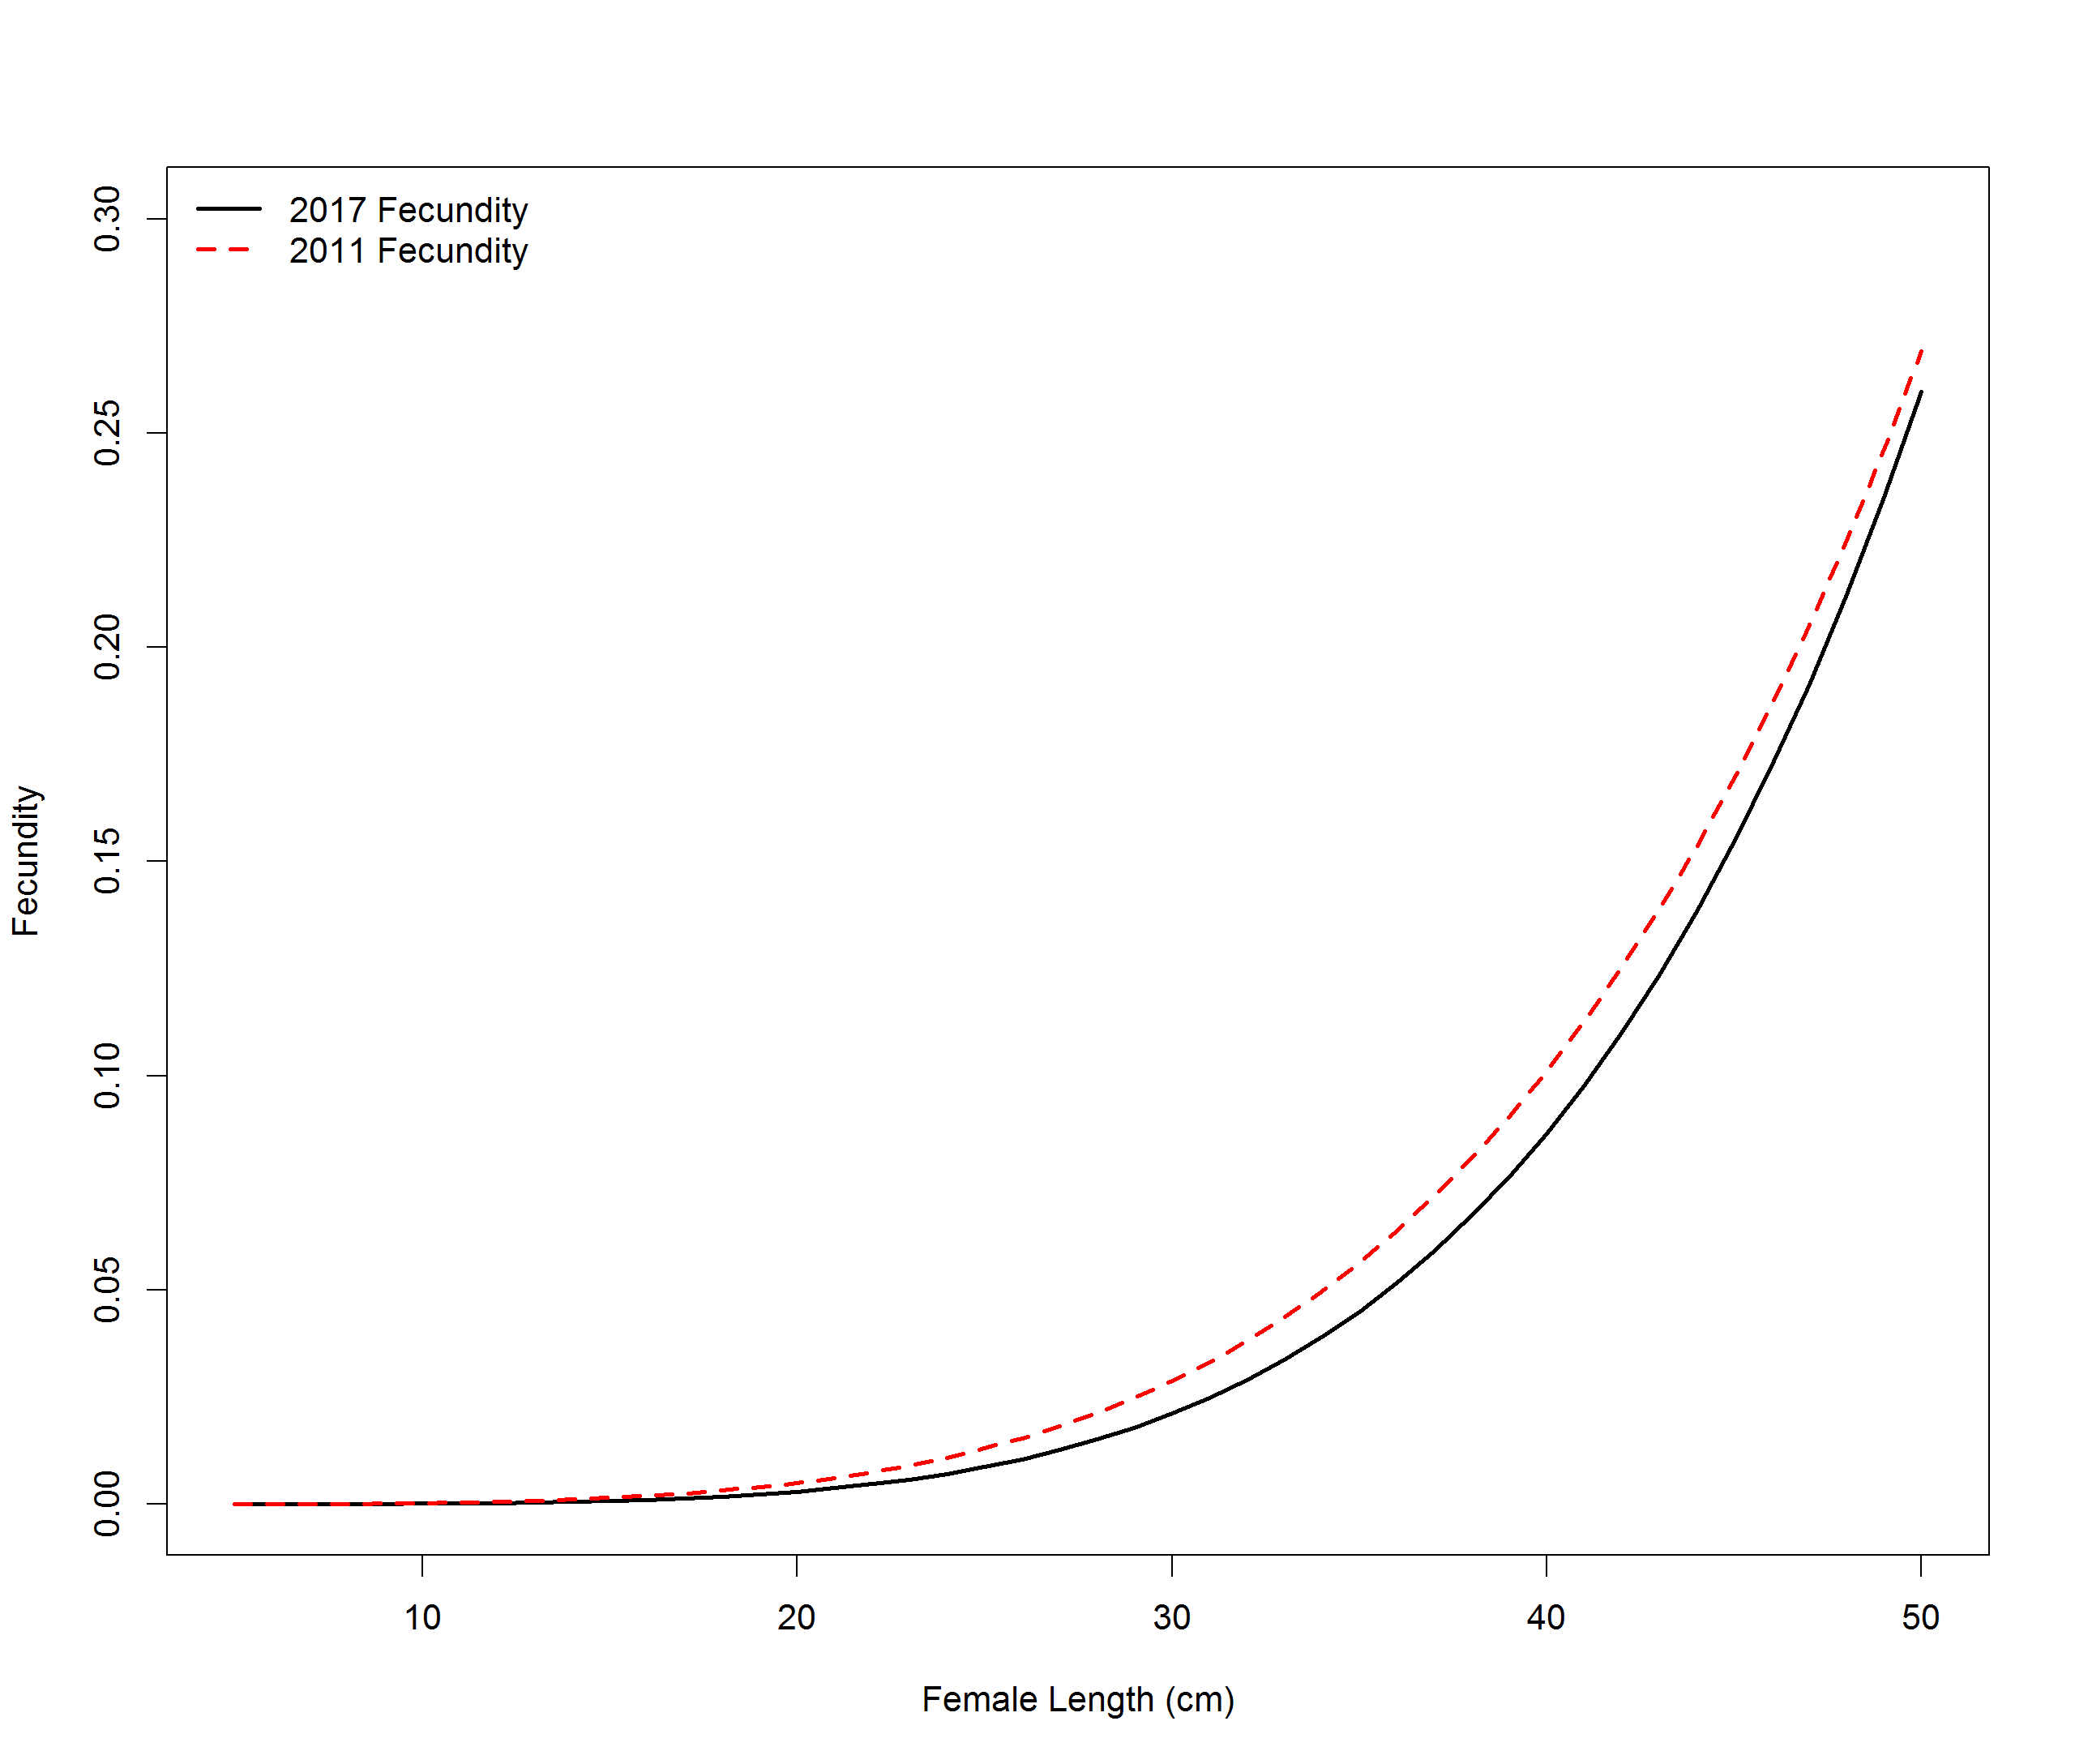
\includegraphics[scale = 0.3, trim={0, 0, 1cm, 1cm}, clip]{figures/Fecundity_Comparison.png}
  \end{center}
  *Sensitivity to assumed fecundity shown to not have a large impact on results
\end{frame}

\subsection{Growth}
\begin{frame}{Weight-at-Length}
  \begin{center}
    %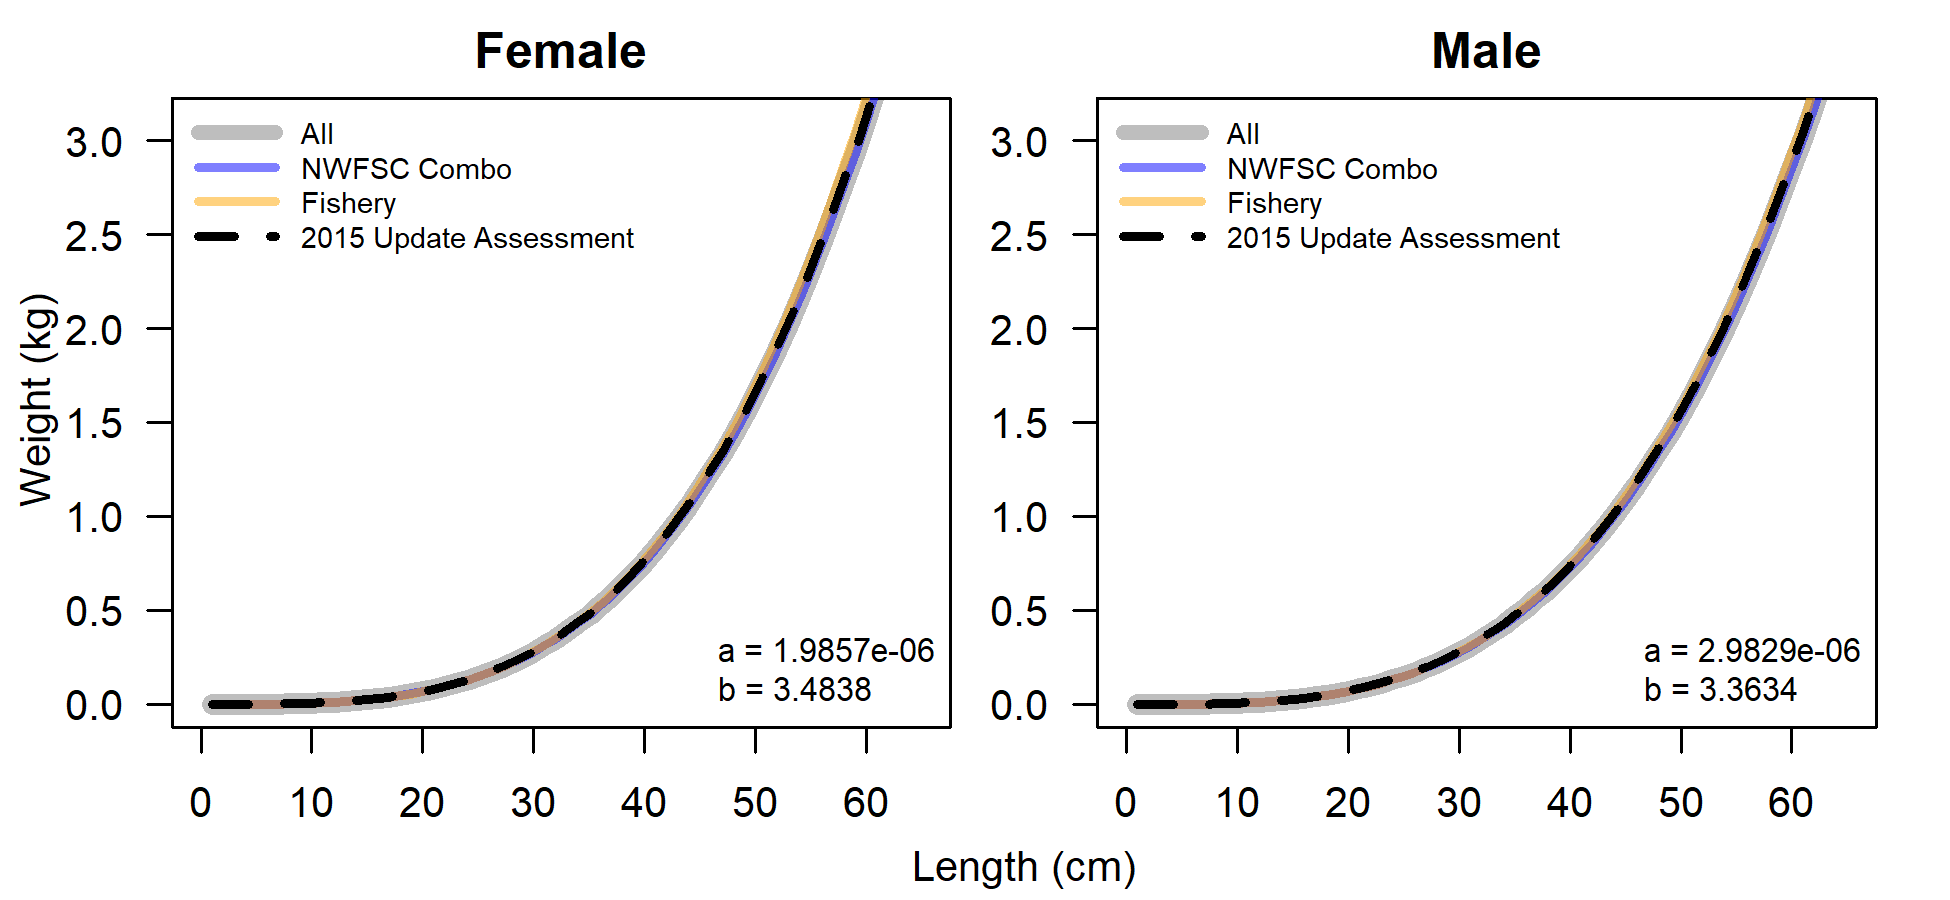
\includegraphics[scale = 0.75]{figures/weightAtLengthPred.png}
  \end{center}
\end{frame}

\begin{frame}{Length-at-Age}
  \begin{center}
  %\includegraphics[scale = 0.45]{figures/LengthAgeAll_2.png}
  \end{center}
\end{frame}


%-------------------------------------------------------------------------------------
%\section{Data Summary}
%-------------------------------------------------------------------------------------

\subsection{}
\begin{frame}{Data Summary Used in the 2017 Assessment}
  \begin{figure}[ht]
    \begin{center}
      %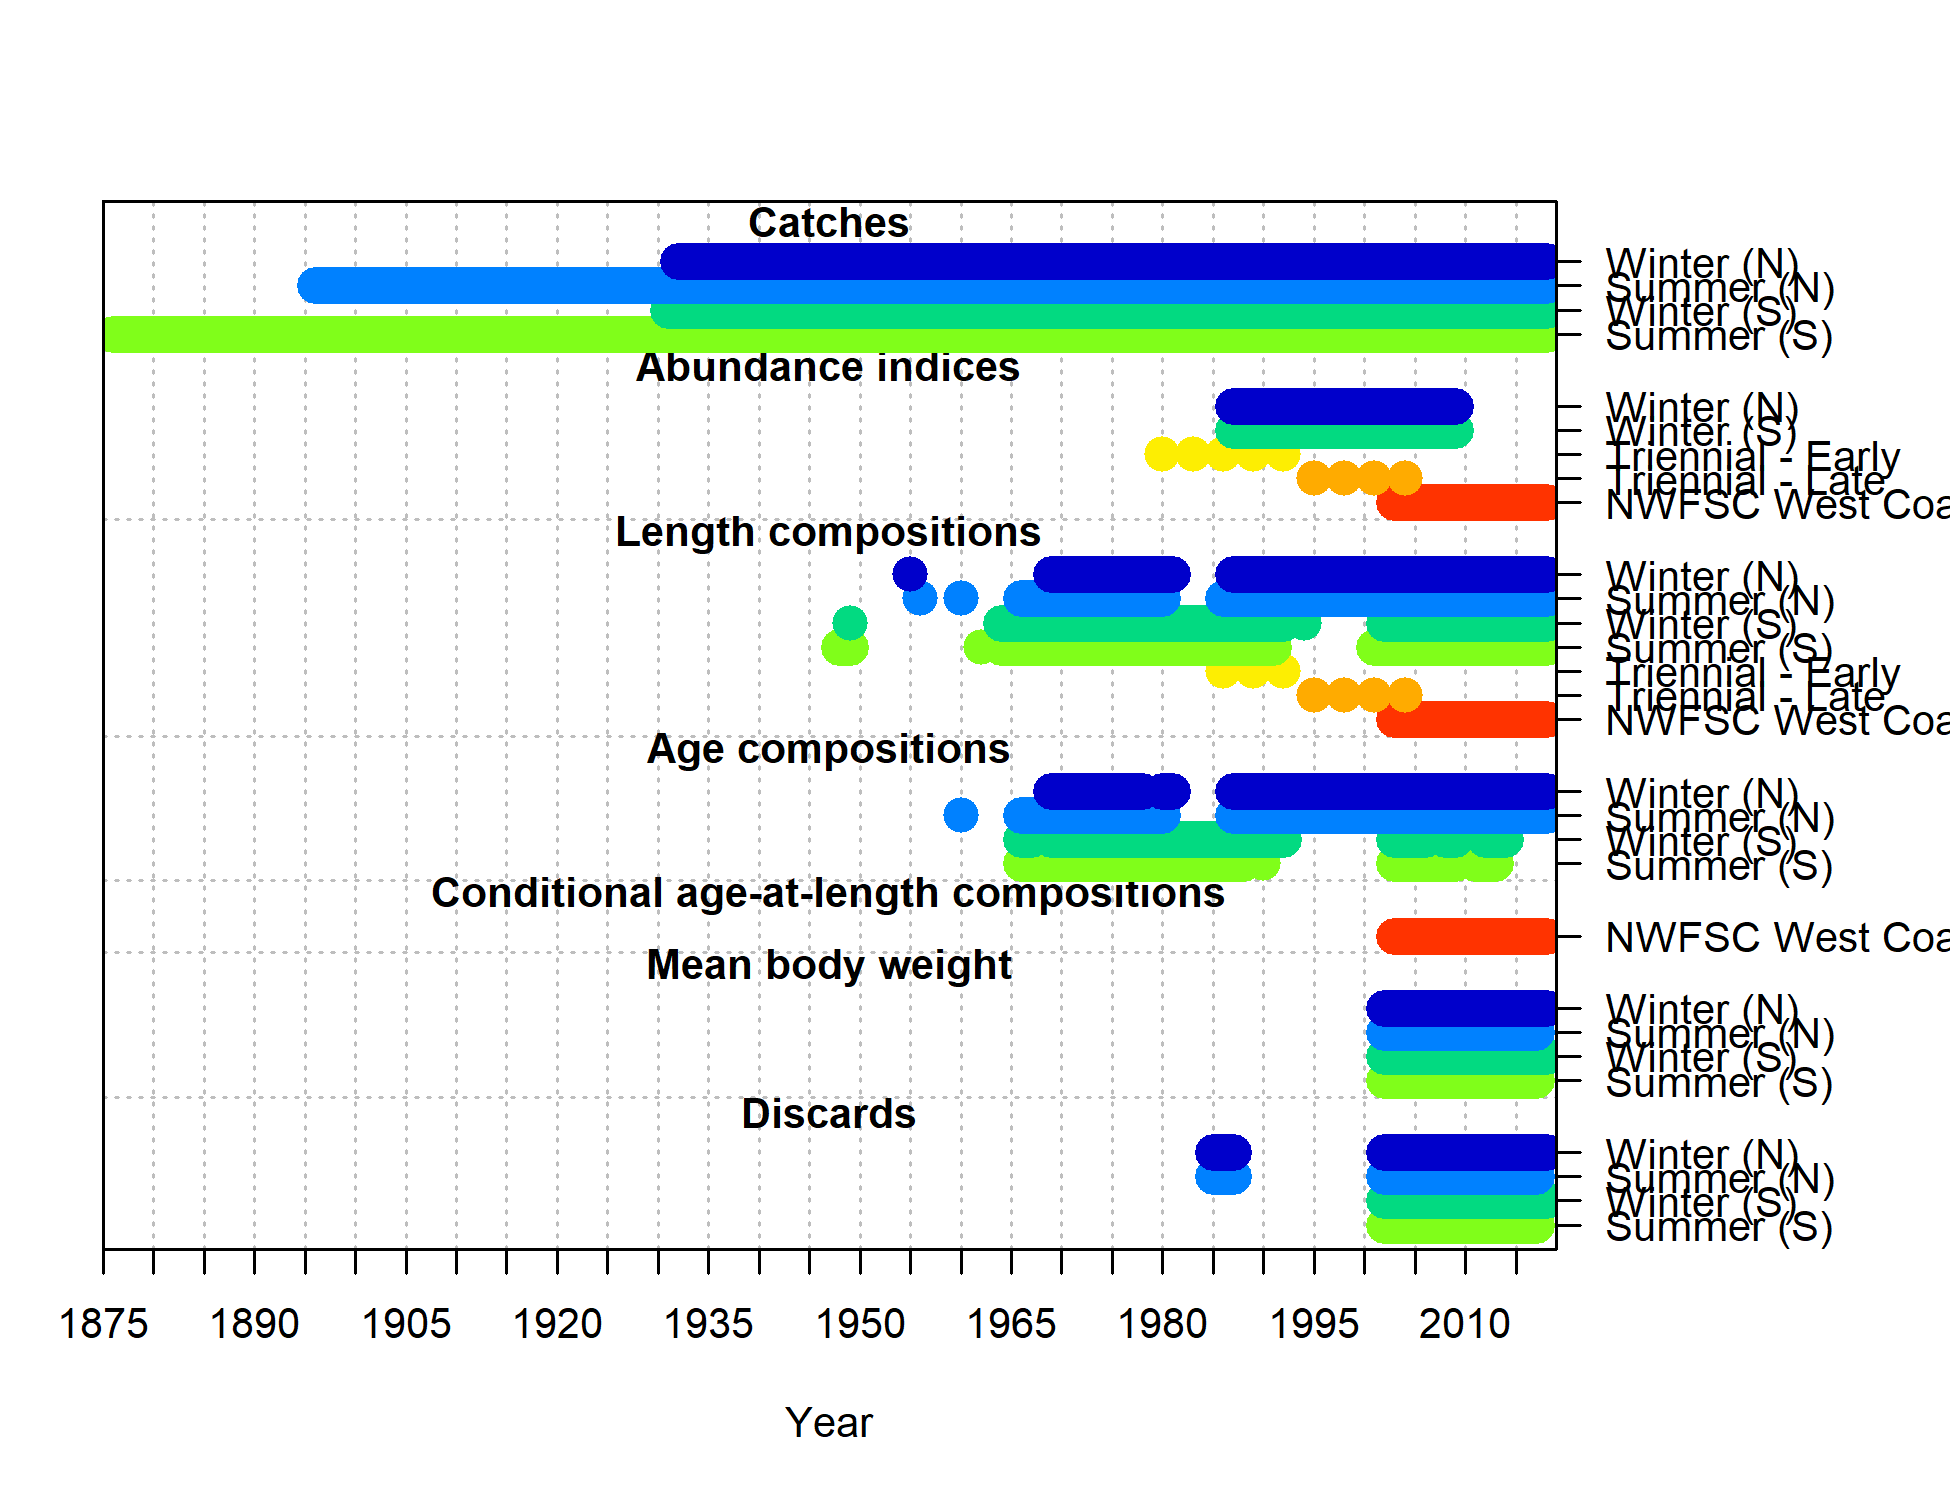
\includegraphics[height=3in]{r4ss/data_plot.png}

    \end{center}
  \end{figure}
\end{frame}


%---------------------------------------------------------------------------------
\section{Removals}
%---------------------------------------------------------------------------------
\subsection{Landings History by State}
\begin{frame}{Landings Data: 2017 vs. 2011}
  \begin{center}
    %\includegraphics[scale = 0.45]{figures/pop2017_2011vs2017catches_states.png}
  \end{center}
\end{frame}

\begin{frame}{Cumulative Catch Difference}
  \begin{center}
    %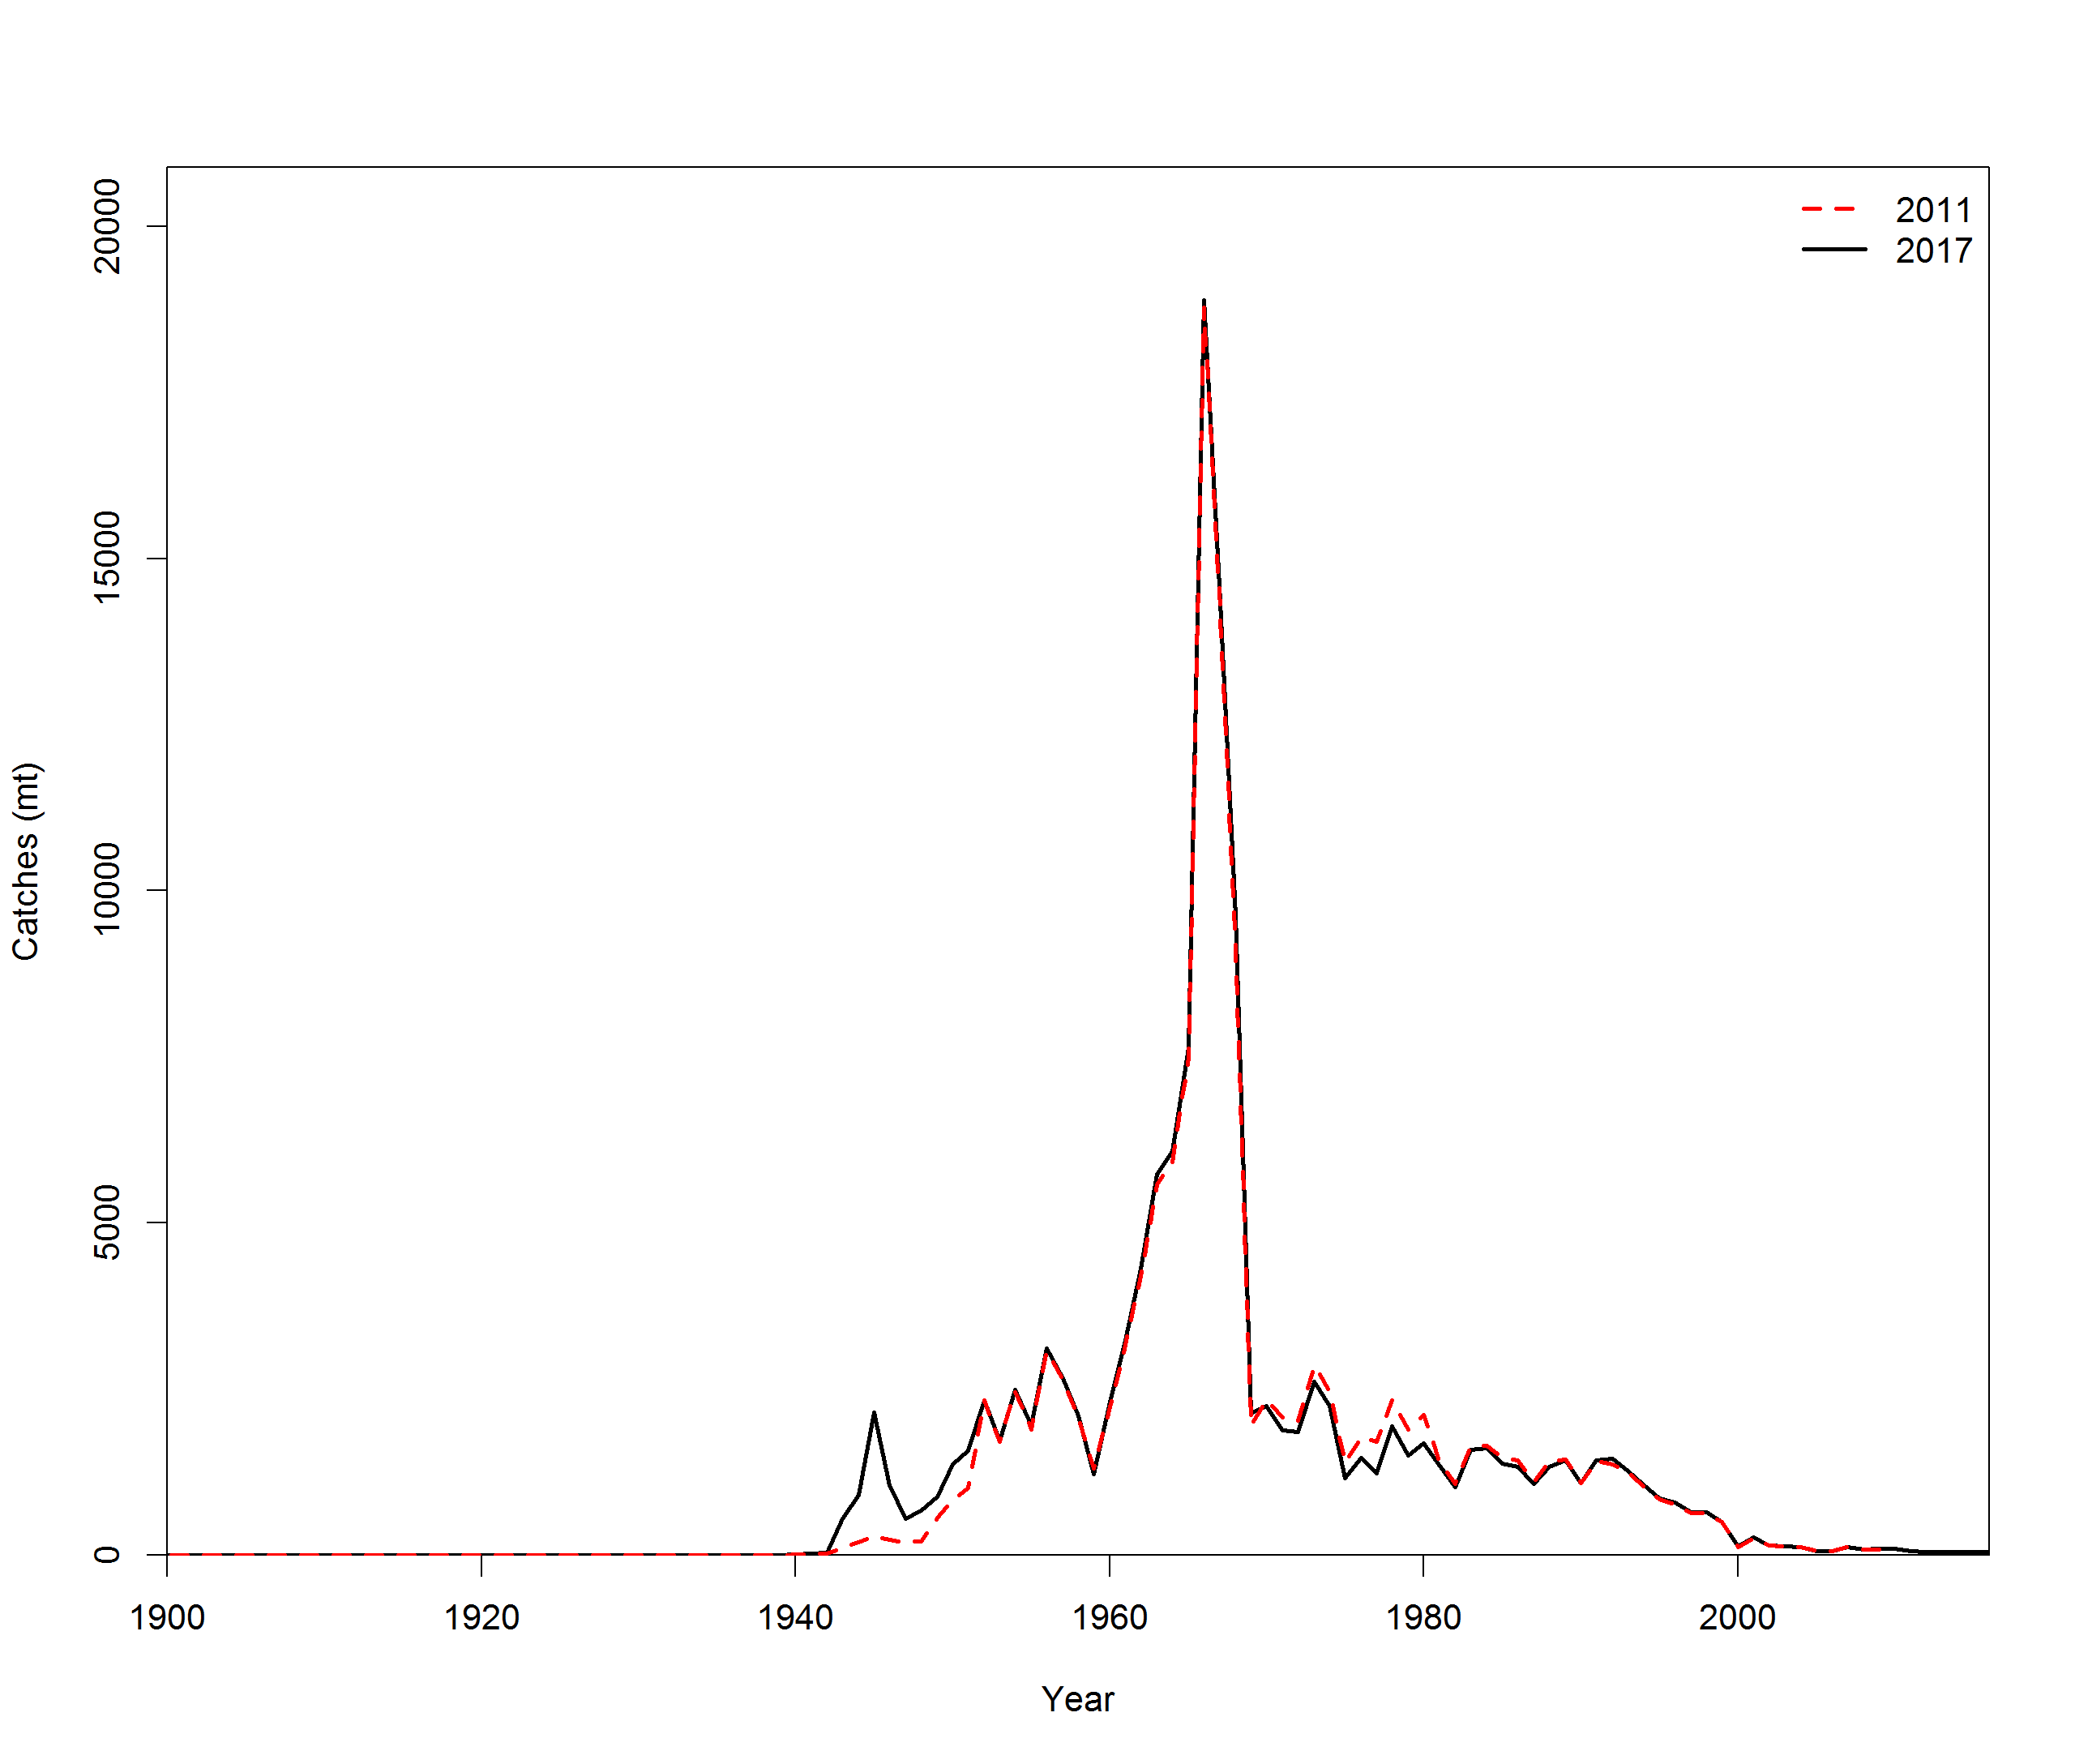
\includegraphics[scale = 0.32, trim={0, 0, 0, 2cm}, clip]{figures/Catch_Comparison.png}
  \end{center}
  *Resulted in $<$ 1\% change in $R0$ 
\end{frame}



%---------------------------------------------------------------------------------
\section{Index Data}
%---------------------------------------------------------------------------------

\subsection{CPUE and Survey Indices}
\begin{frame}{Survey Stratificaiton and Model Selection}
  \begin{table}[ht]
  \small
  \centering
  \begin{tabular}{p{1.15in}p{0.65in}p{0.5in}p{0.5in}p{0.75in}}
  Survey & Depth (m) & Latitude & Model & Error  \\ 
  \hline
  Pacific ocean perch & 155-500 & 44-48.5 & VAST & Lognormal \\
  Triennial shelf & 55-366 & 40.5-49 & VAST & Lognormal\\ 
  AFSC slope & 183-549 & 42-49 & VAST & Lognormal \\ 
  NWFSC slope & 183-549 & 42-49 & Bayesian delta glmm & Gamma \\
  NWFSC shelf-slope & 55-549 & 42-49 & VAST & Lognormal \\
  \hline
  \end{tabular}
  \end{table}
\end{frame}


\begin{frame}{Designed Based vs. Model Indices}
  \begin{center}
    %\includegraphics[scale = 0.30]{figures/Index_DesignBased_Comparison.png}
  \end{center}
\end{frame}

\begin{frame}{Pacific Ocean Perch Survey Diagnostics}
  \begin{center}
  %\includegraphics[scale = 0.50]{figures/POP_Q-Q_plot.jpg}
  %\includegraphics[scale = 0.50]{figures/POP_Q-Q_hist.jpg}
  \end{center}
\end{frame}

\begin{frame}{Triennial Shelf Survey Diagnostics}
  \begin{center}
  %\includegraphics[scale = 0.50]{figures/Tri_Q-Q_plot.jpg}
  %\includegraphics[scale = 0.50]{figures/Tri_Q-Q_hist.jpg}
  \end{center}
\end{frame}


\begin{frame}{All: Standardized}
  \begin{center}
  %\includegraphics[scale = 0.37]{figures/Index_Standardized.png}
  \end{center}
\end{frame}


%---------------------------------------------------------------------------------
\section{Composition Data}
%---------------------------------------------------------------------------------
\subsection{Fishery Data}
\begin{frame}{Fishery Length and Age Data}
  Fishery length data used in the 2017 assessment:
  \begin{itemize}
    \item Fishery: bottom trawl, mid-water trawl, fixed gear
      \begin{itemize}
        \item Retained Lengths: 1966-2016
        \item Discarded Lengths: 1986 (Pikitch), 2004-2015
        \item Ages: 1981-1988, 1994, 1999-2016
      \end{itemize}
    \item At-sea hake fishery
      \begin{itemize}
        \item All (Retained and Discarded) Lengths: 2003-2016
        \item Ages: 2003, 2006, 2007, 2014
      \end{itemize}
  \end{itemize}
\end{frame}


\begin{frame}{NWFSC shelf-slope survey }
  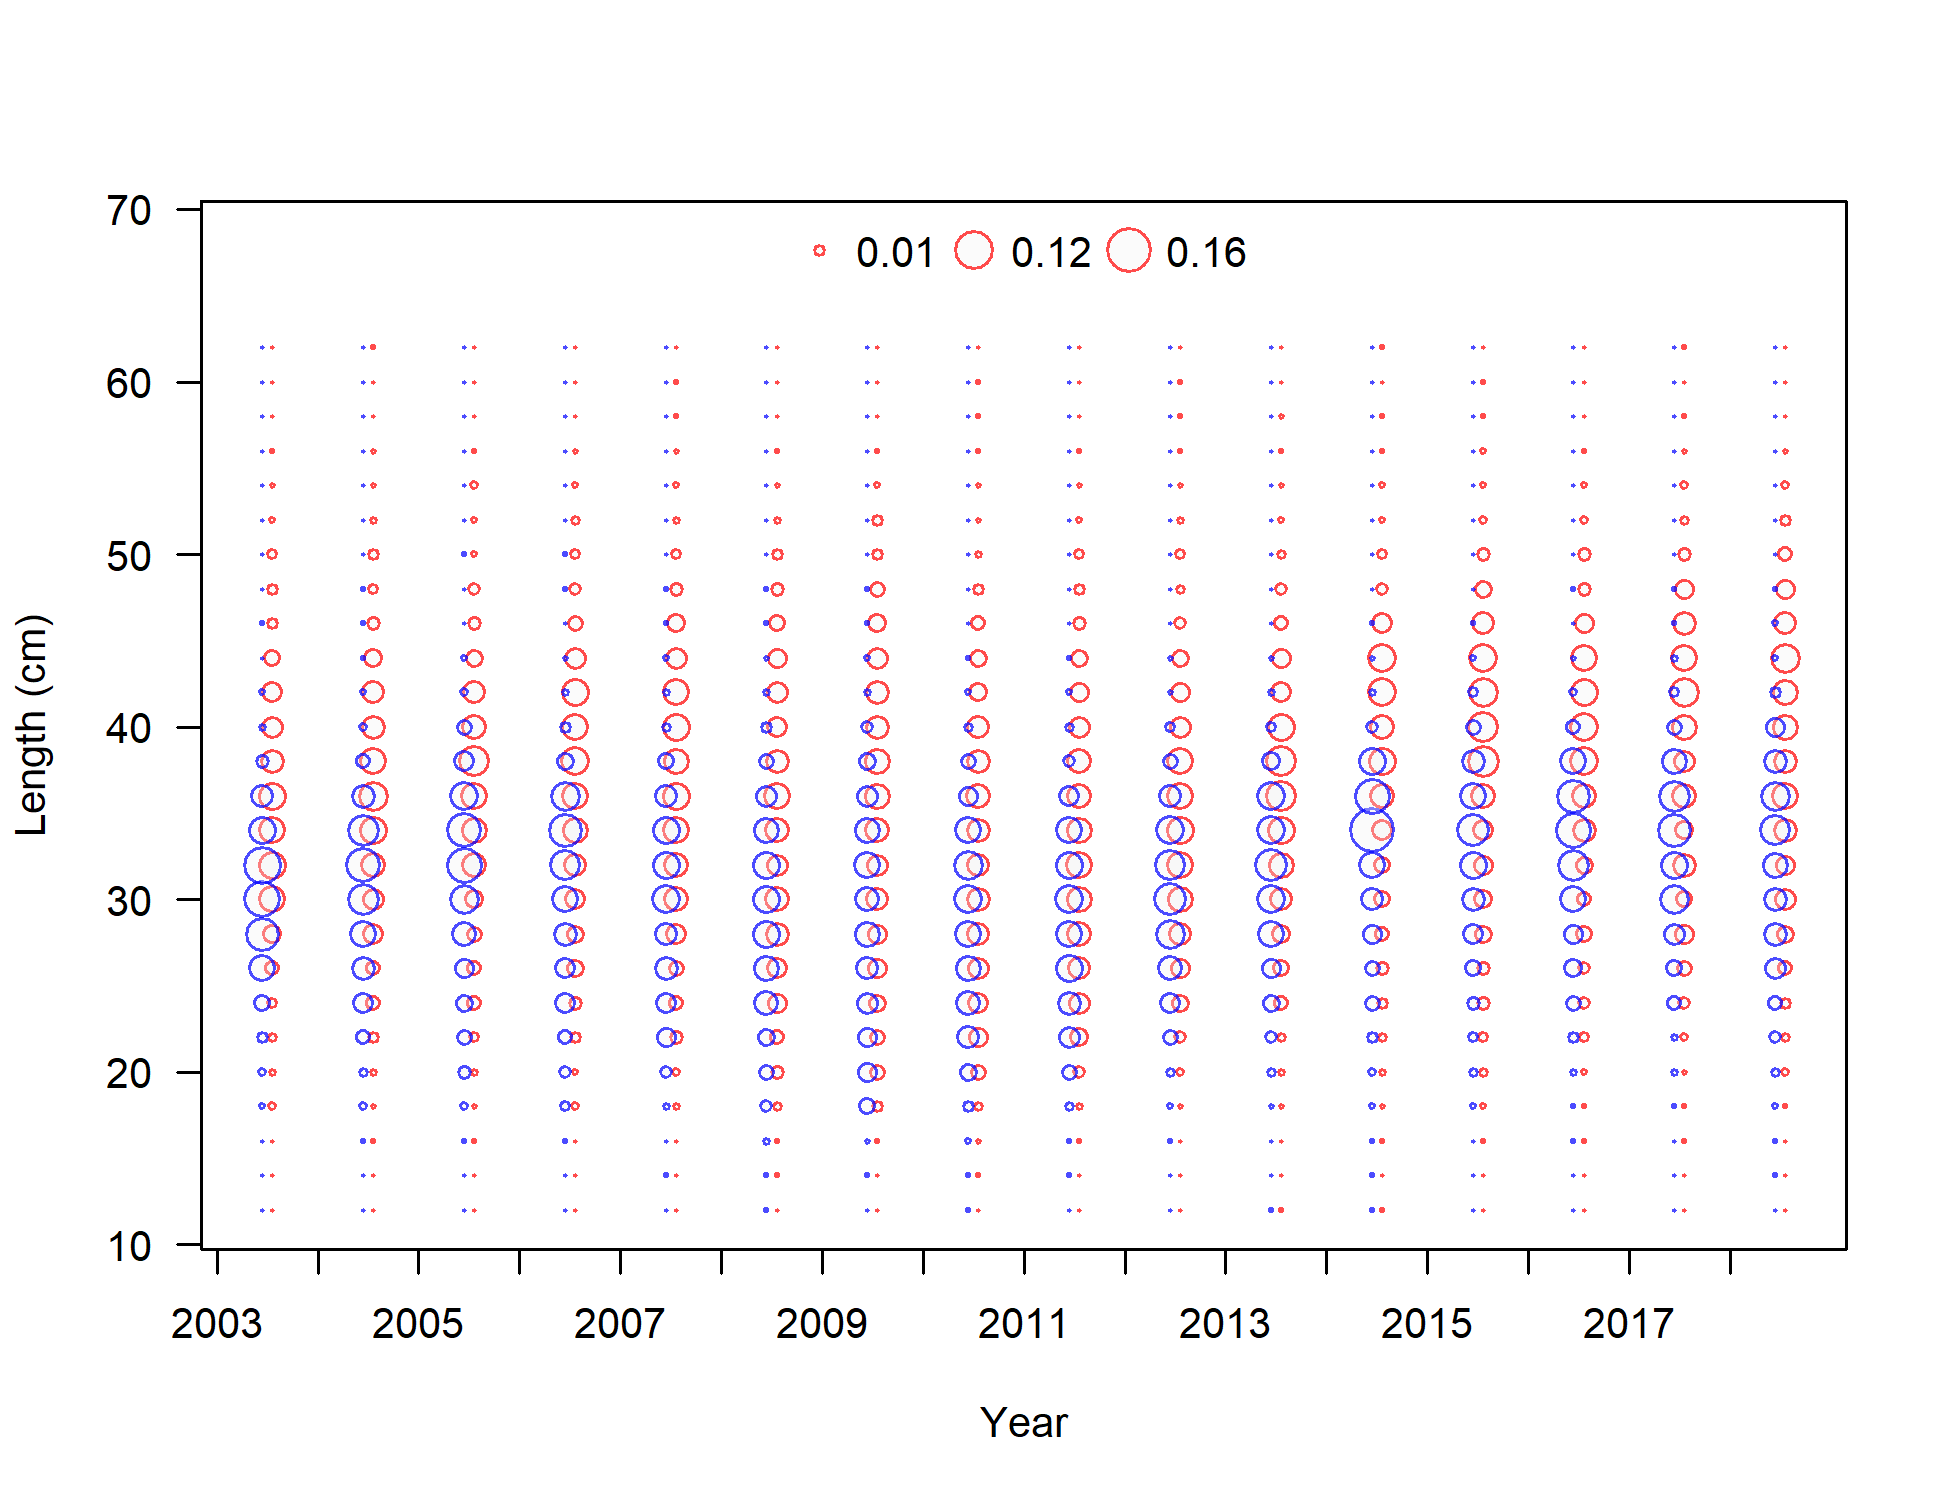
\includegraphics[scale = 0.37]{r4ss/comp_lendat_bubflt7mkt0.png}
  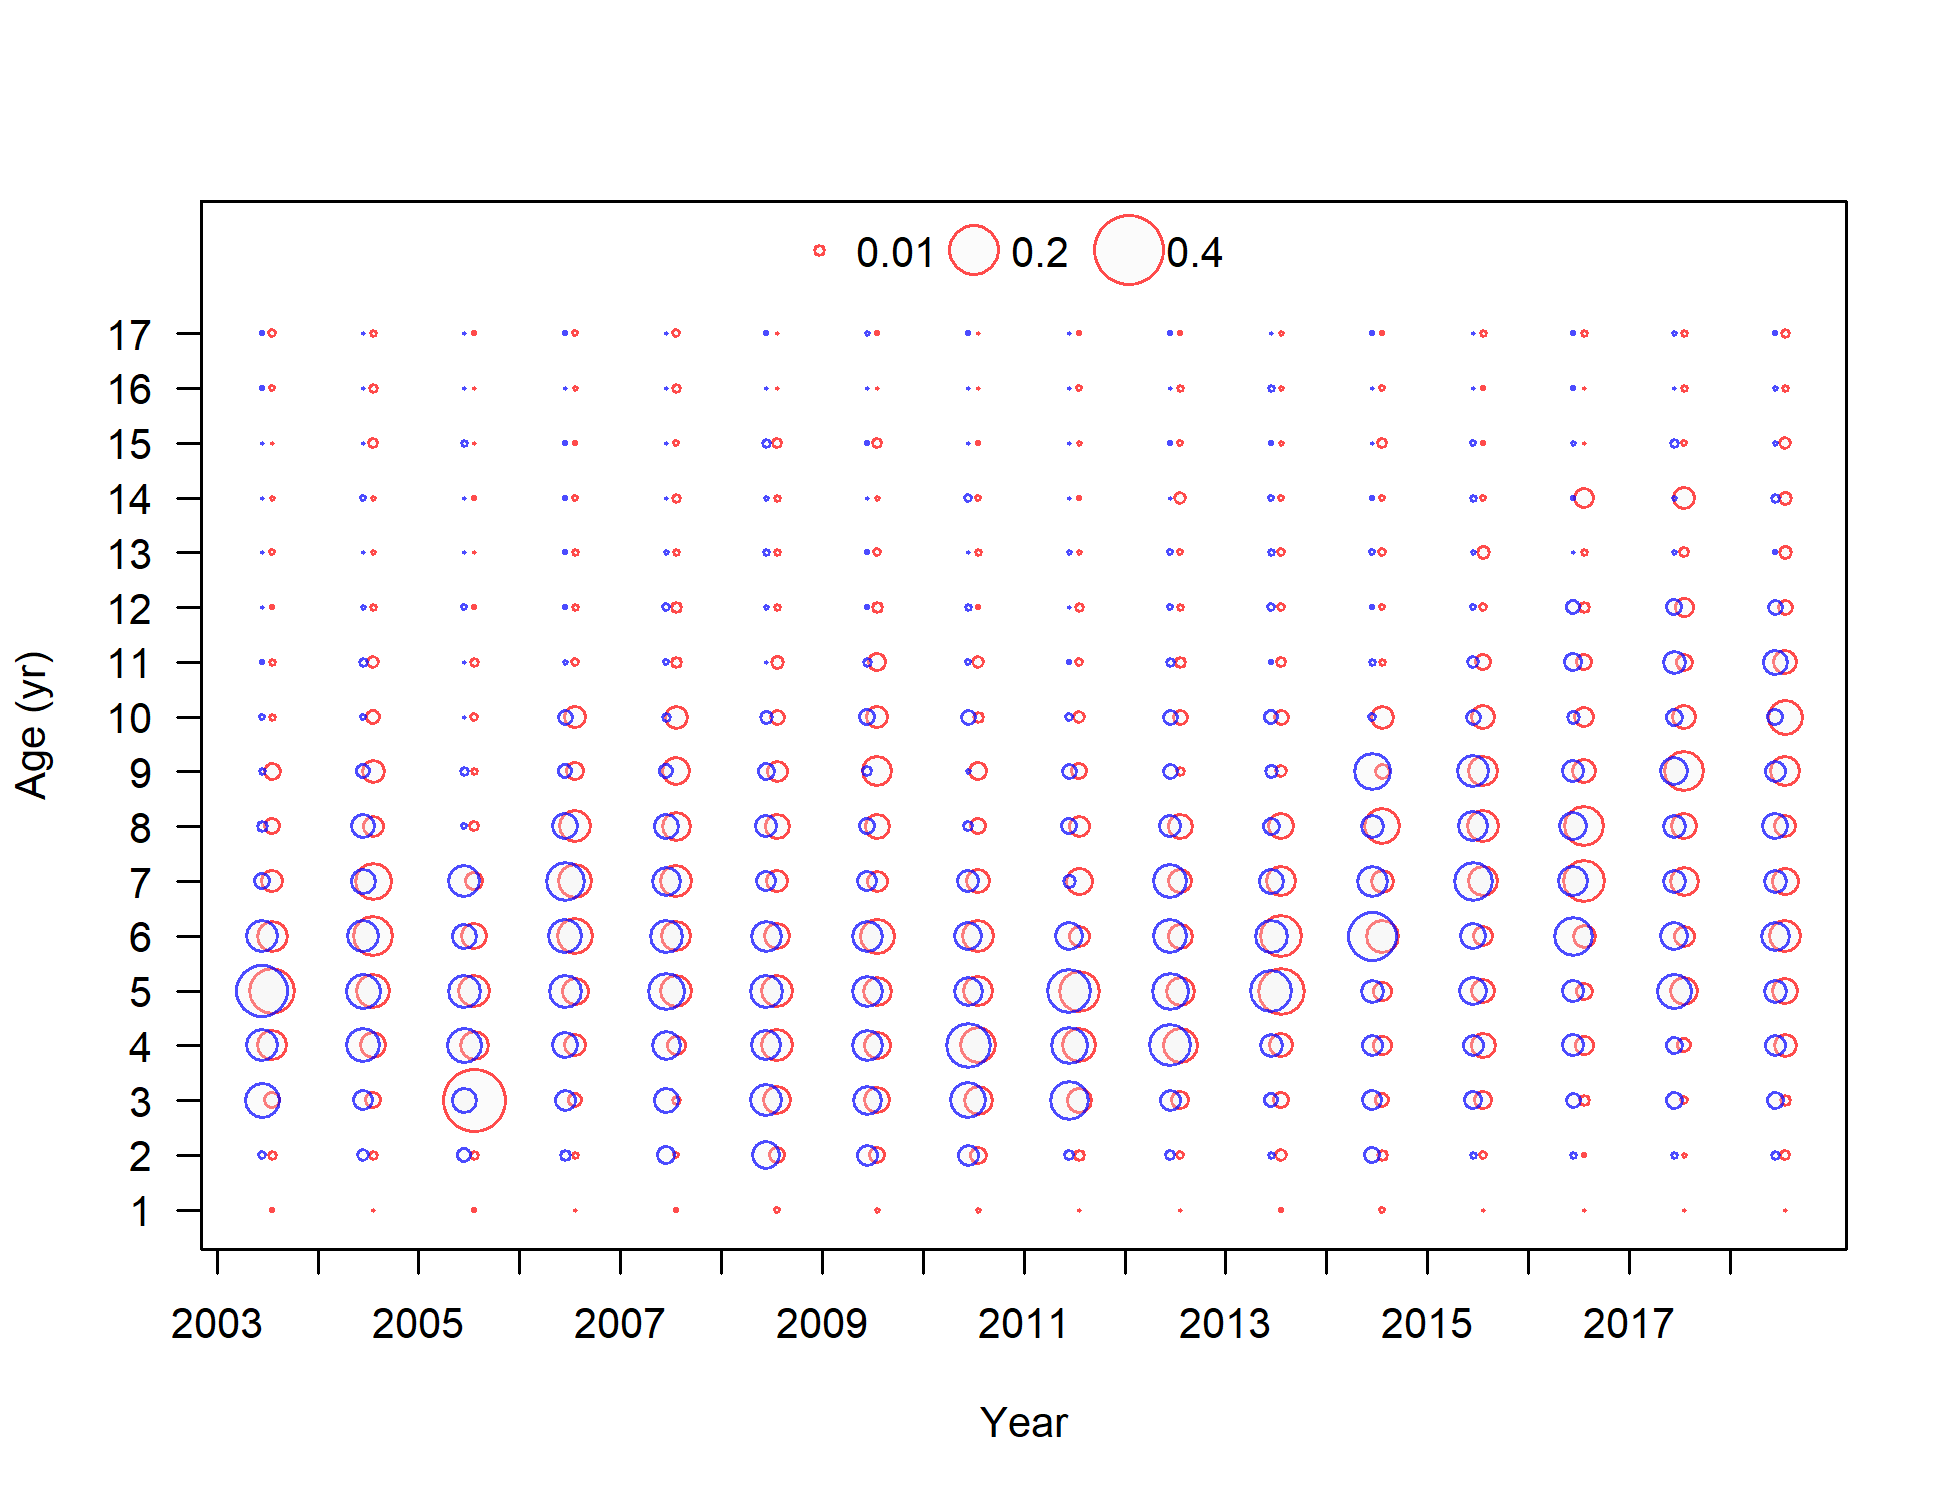
\includegraphics[scale = 0.37]{r4ss/comp_gstagedat_bubflt7mkt0.png}
\end{frame}


\begin{frame}{NWFSC shelf-slope conditional age-at-length}
    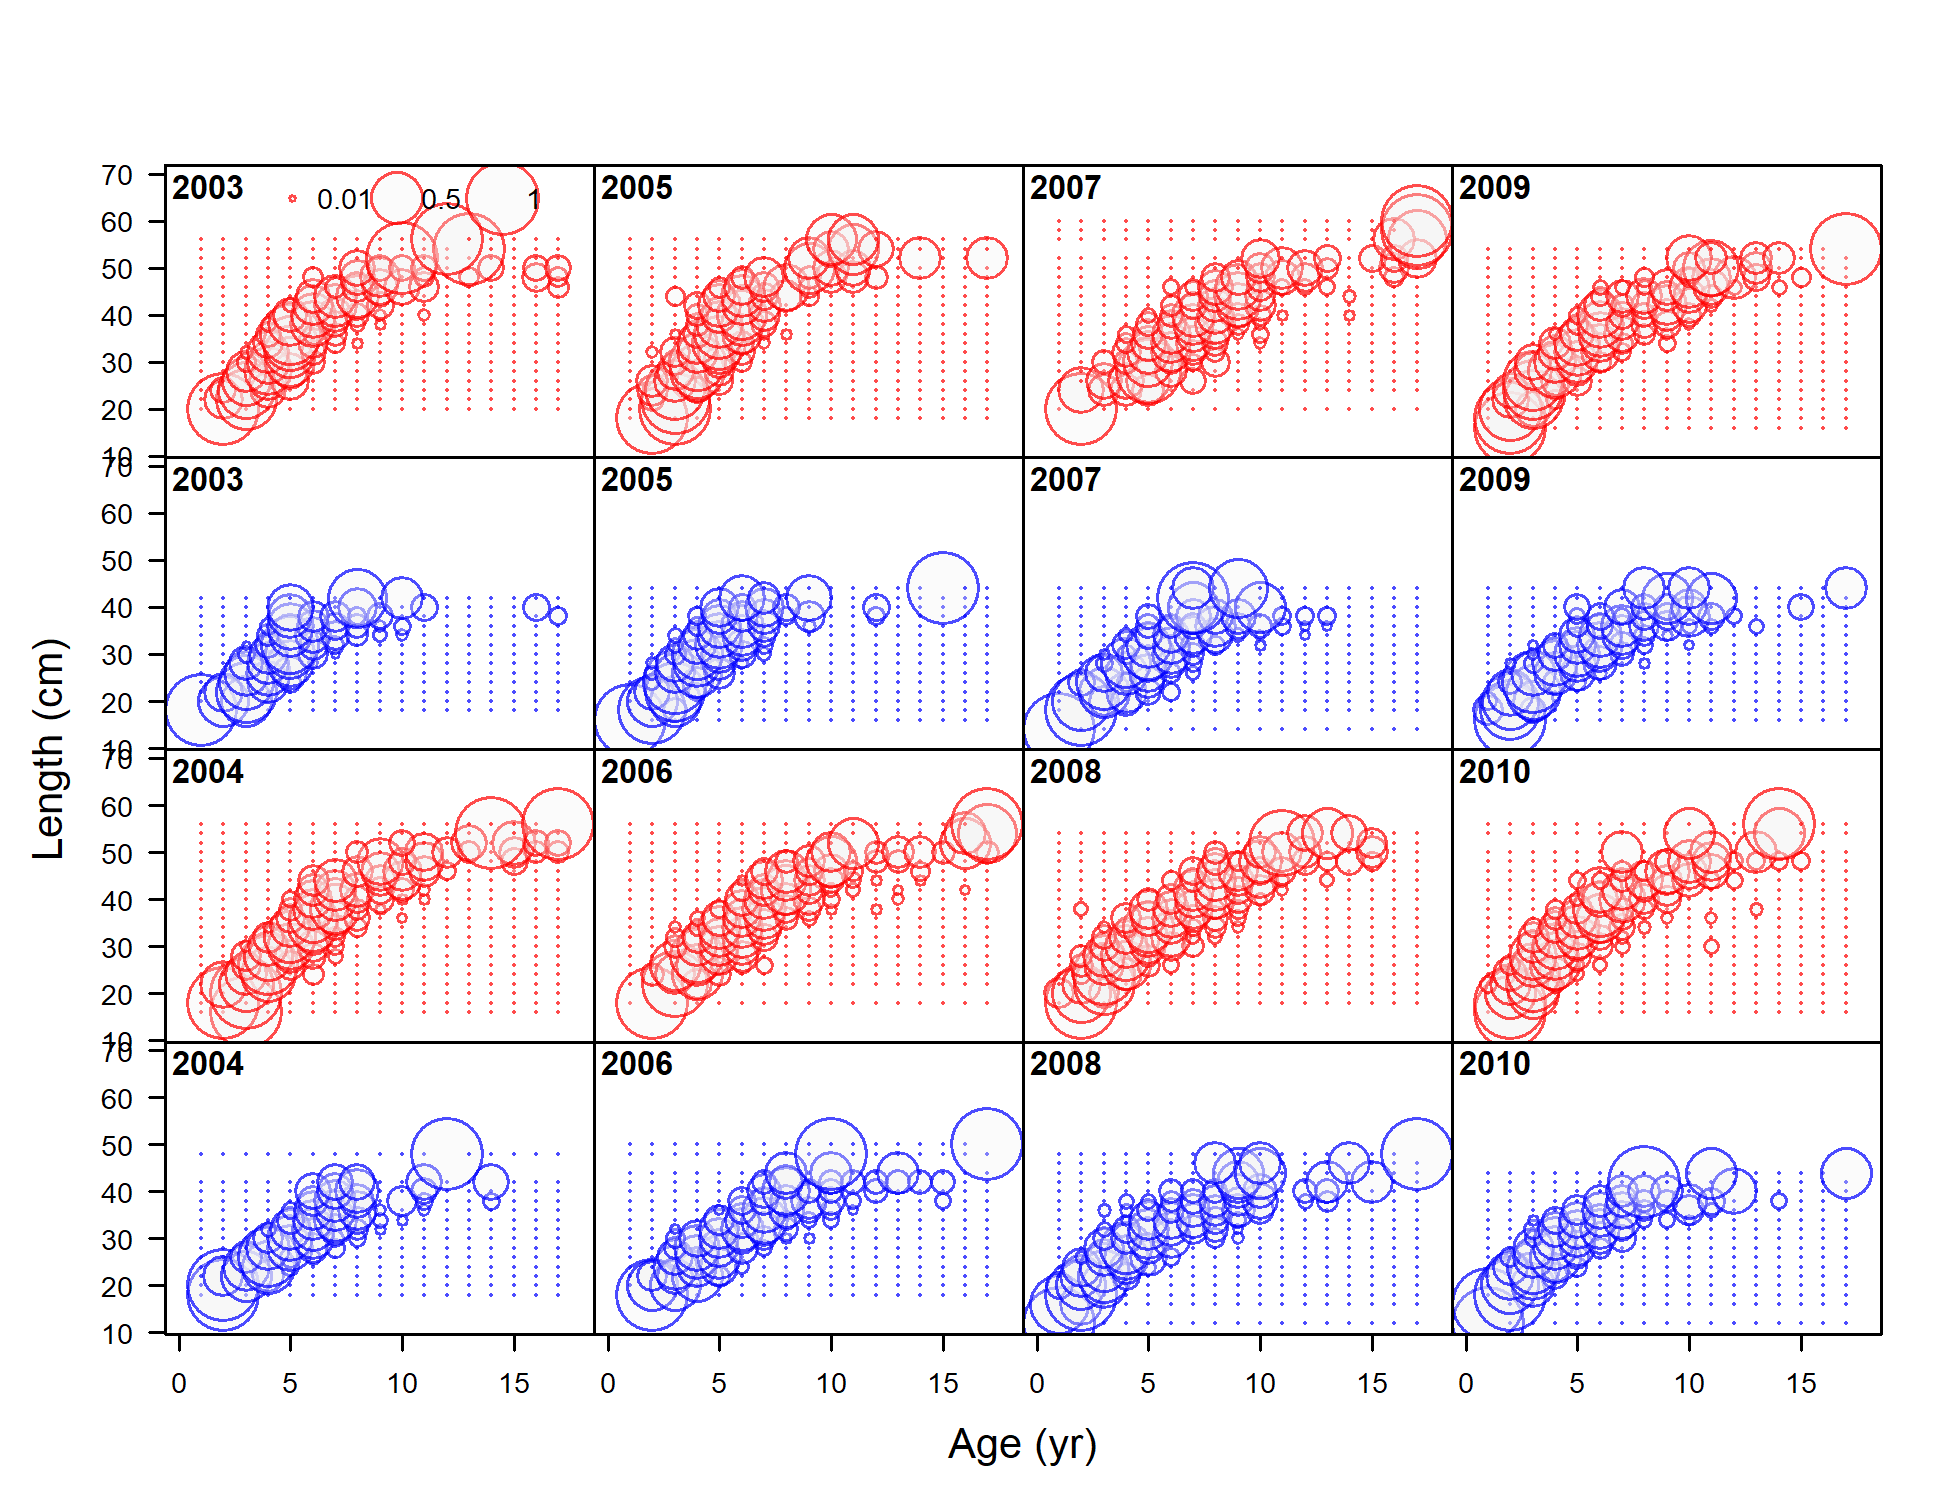
\includegraphics[scale = 0.42]{r4ss/comp_condAALdat_bubflt7mkt0_page1.png}
    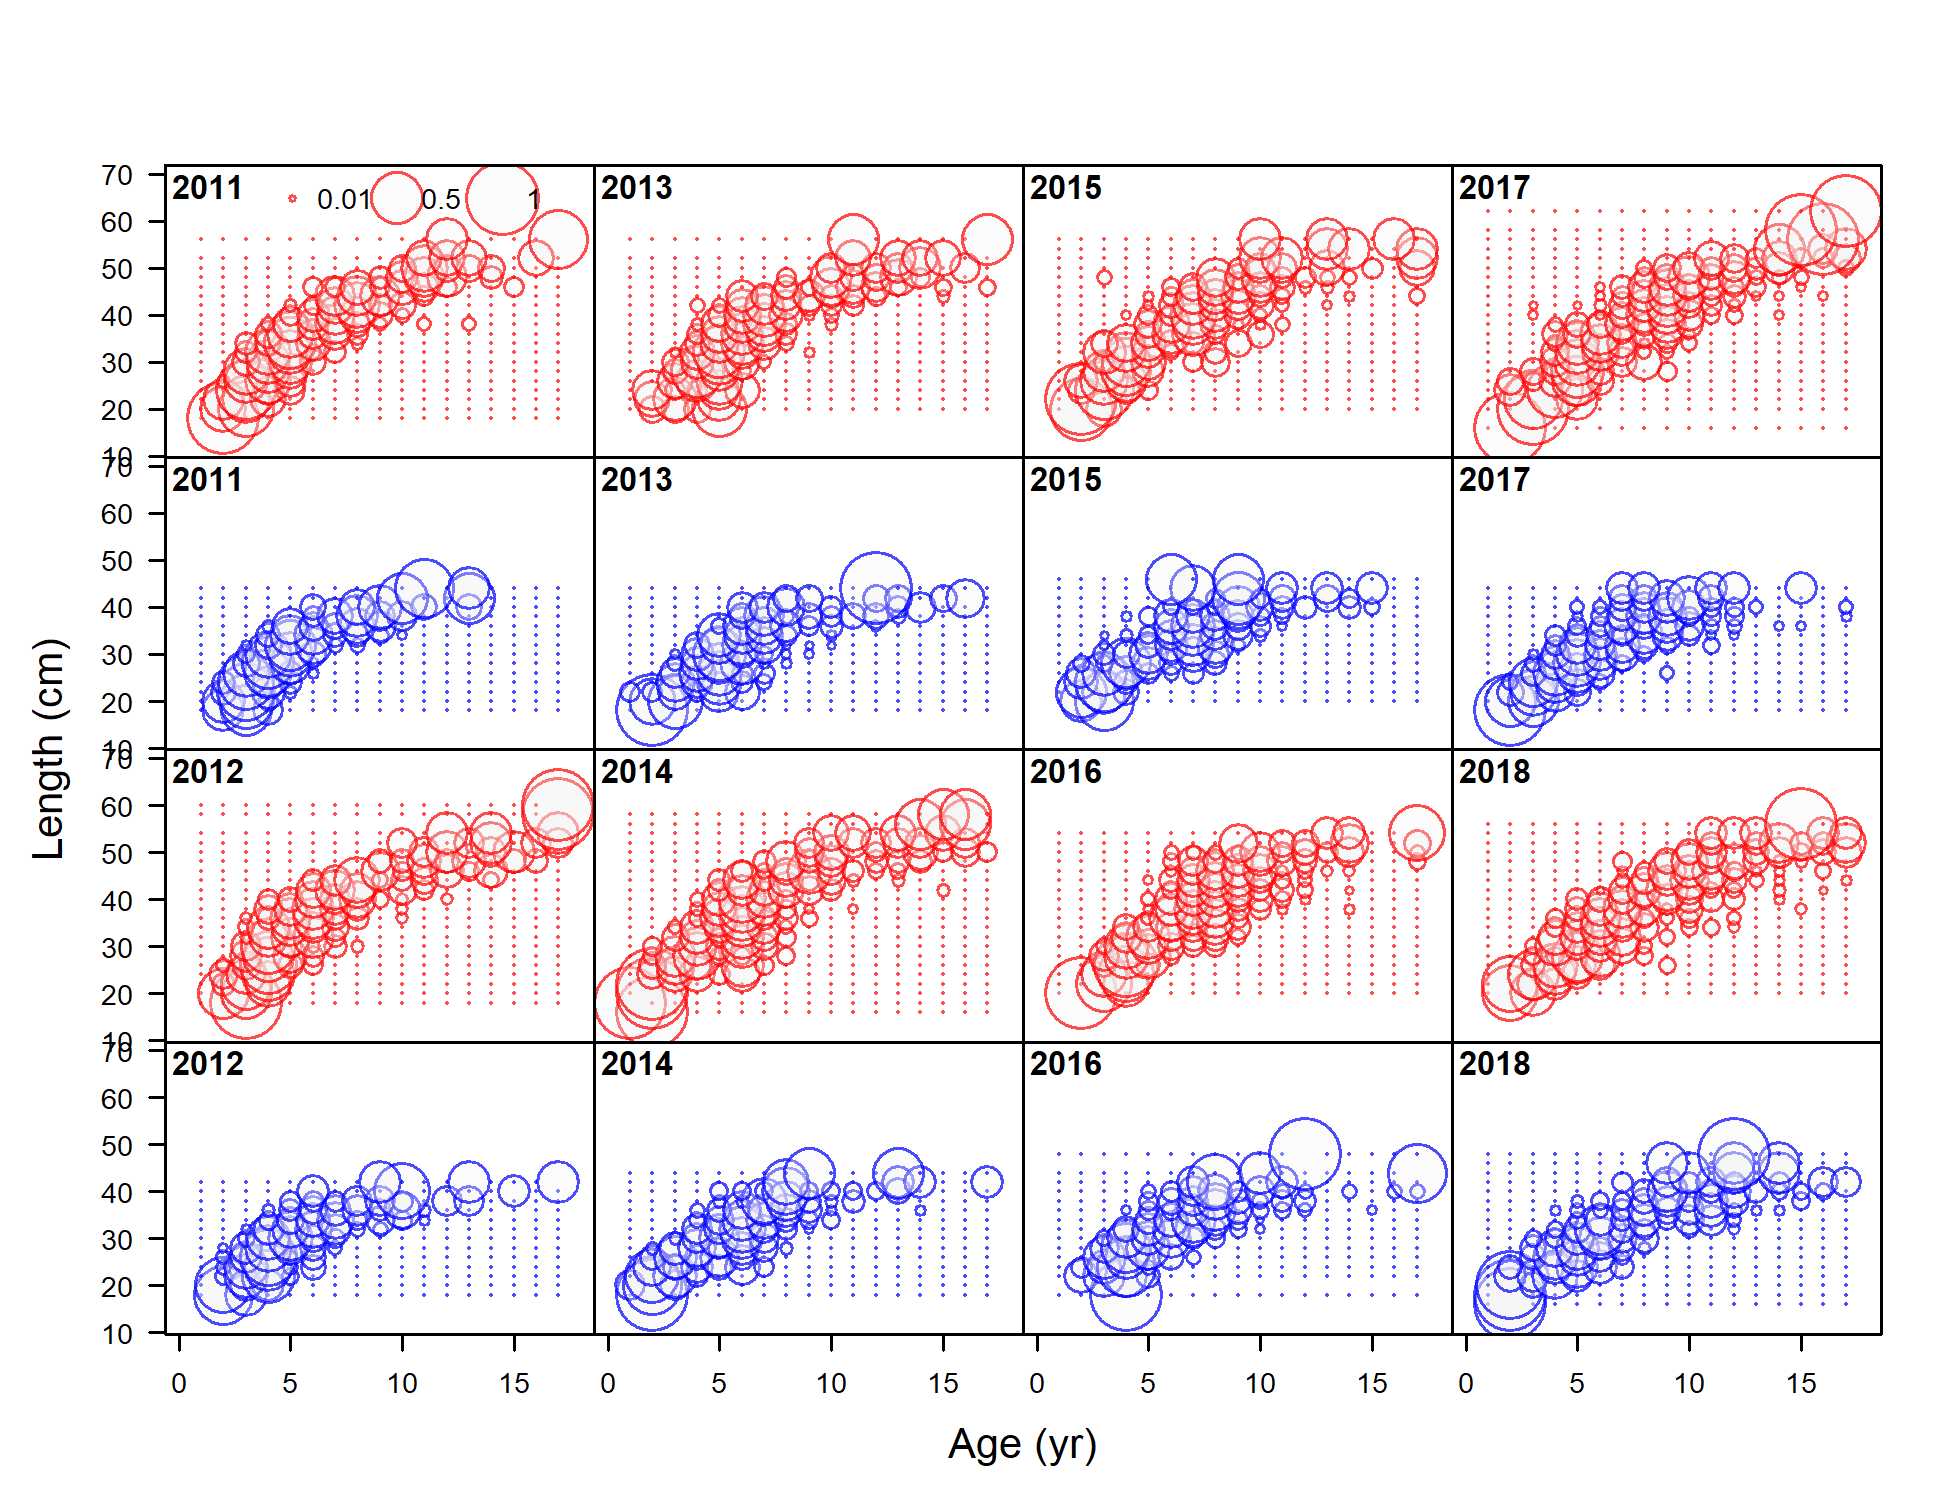
\includegraphics[scale = 0.42]{r4ss/comp_condAALdat_bubflt7mkt0_page2.png}
\end{frame}


\begin{frame}{Aggregated data by source}
    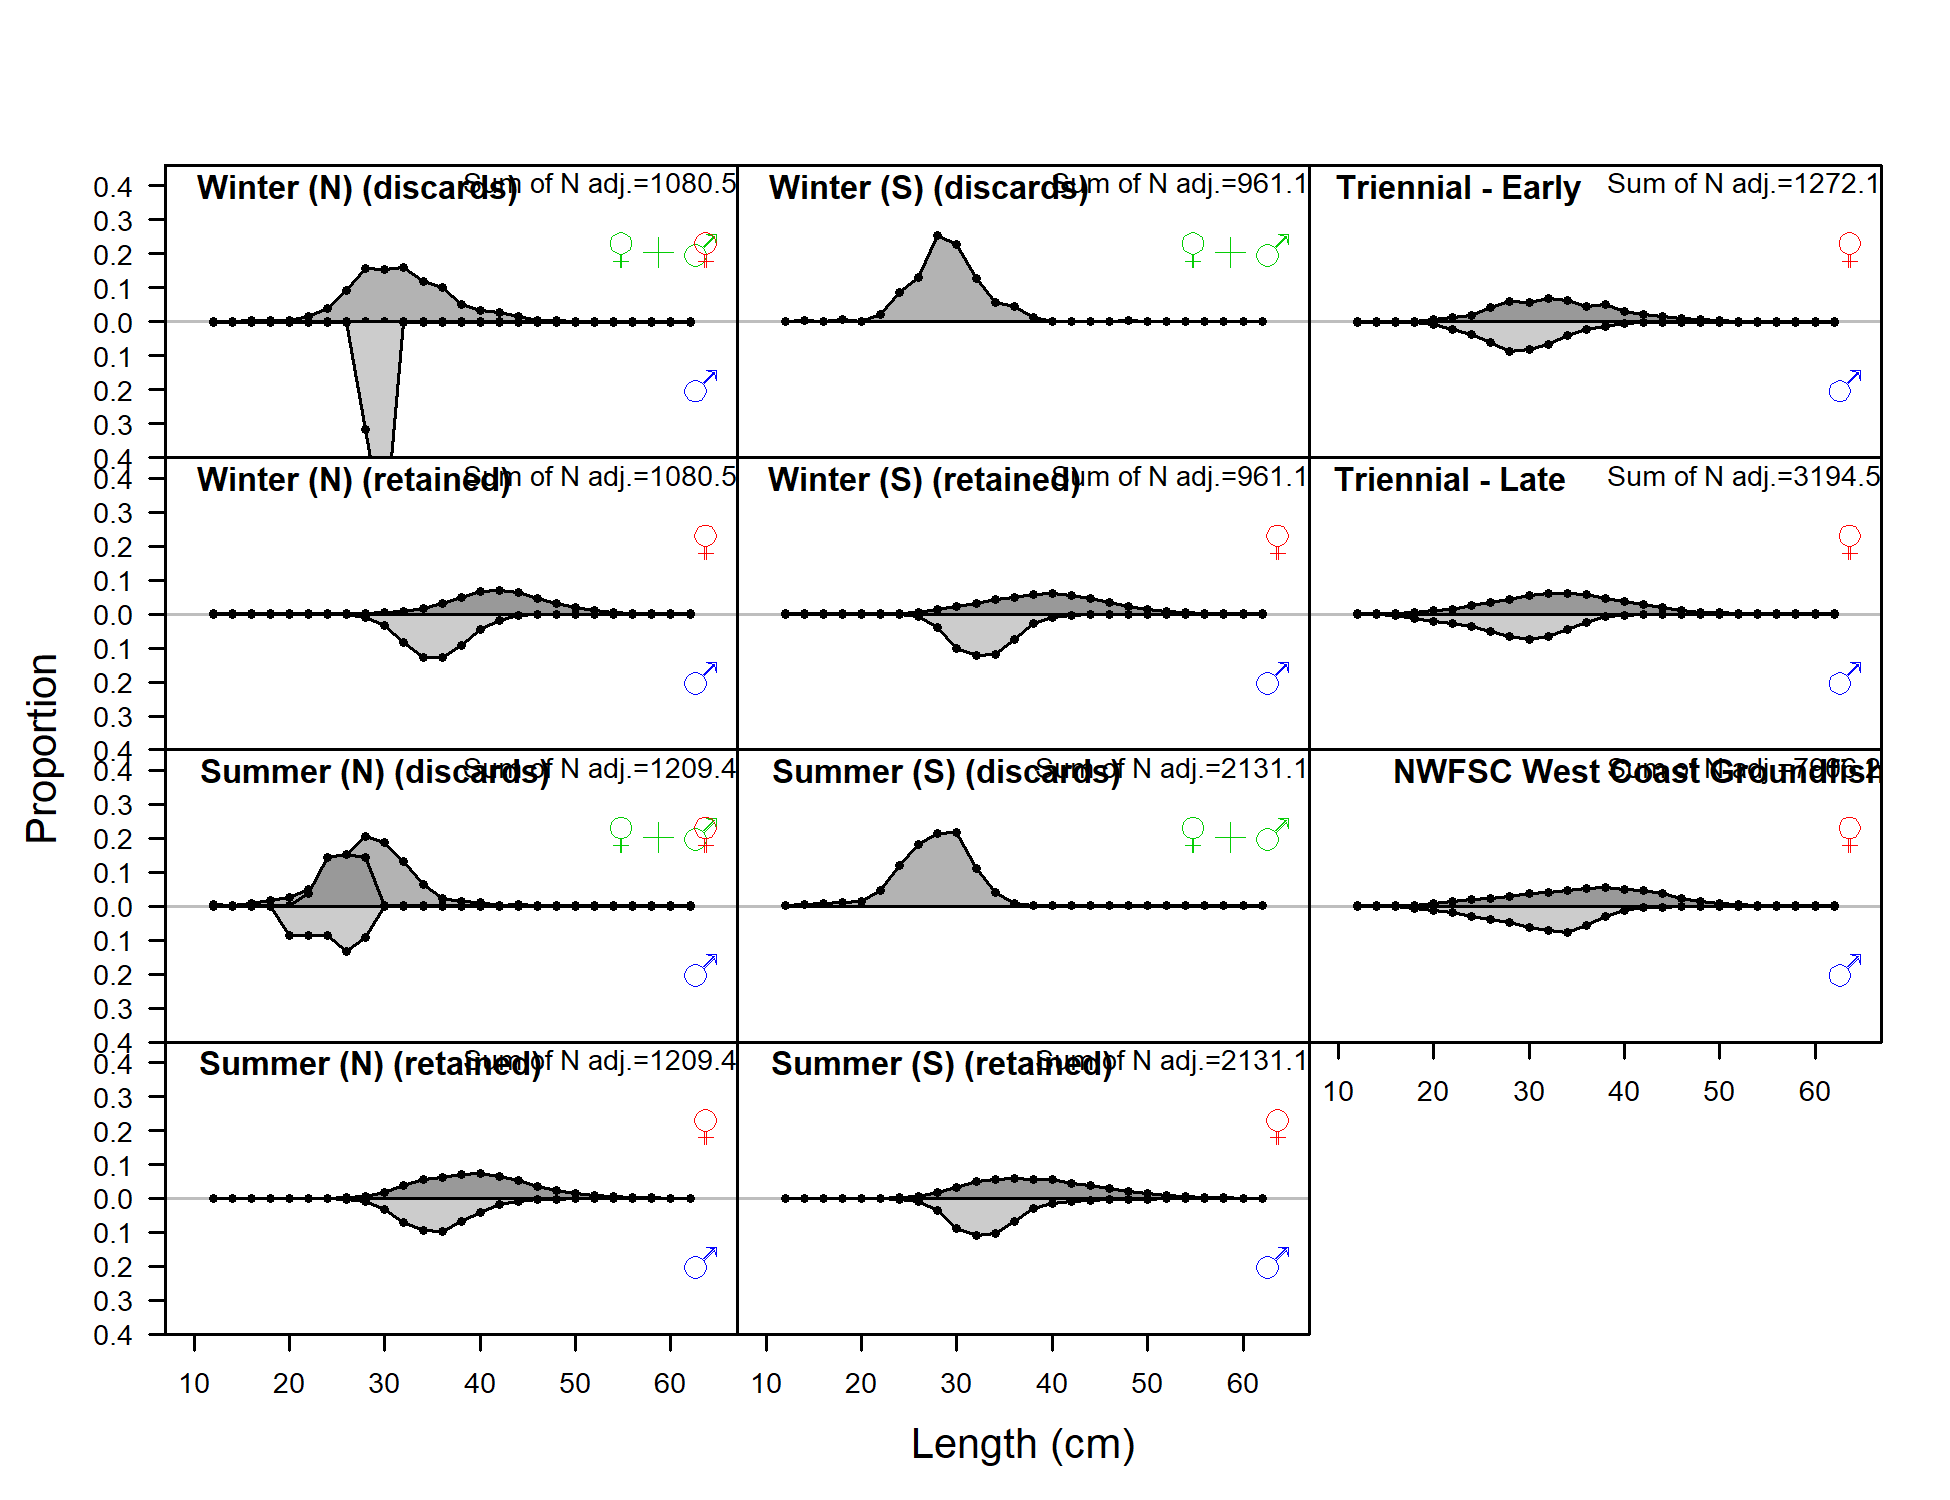
\includegraphics[scale = 0.37]{r4ss/comp_lendat__aggregated_across_time.png}
    %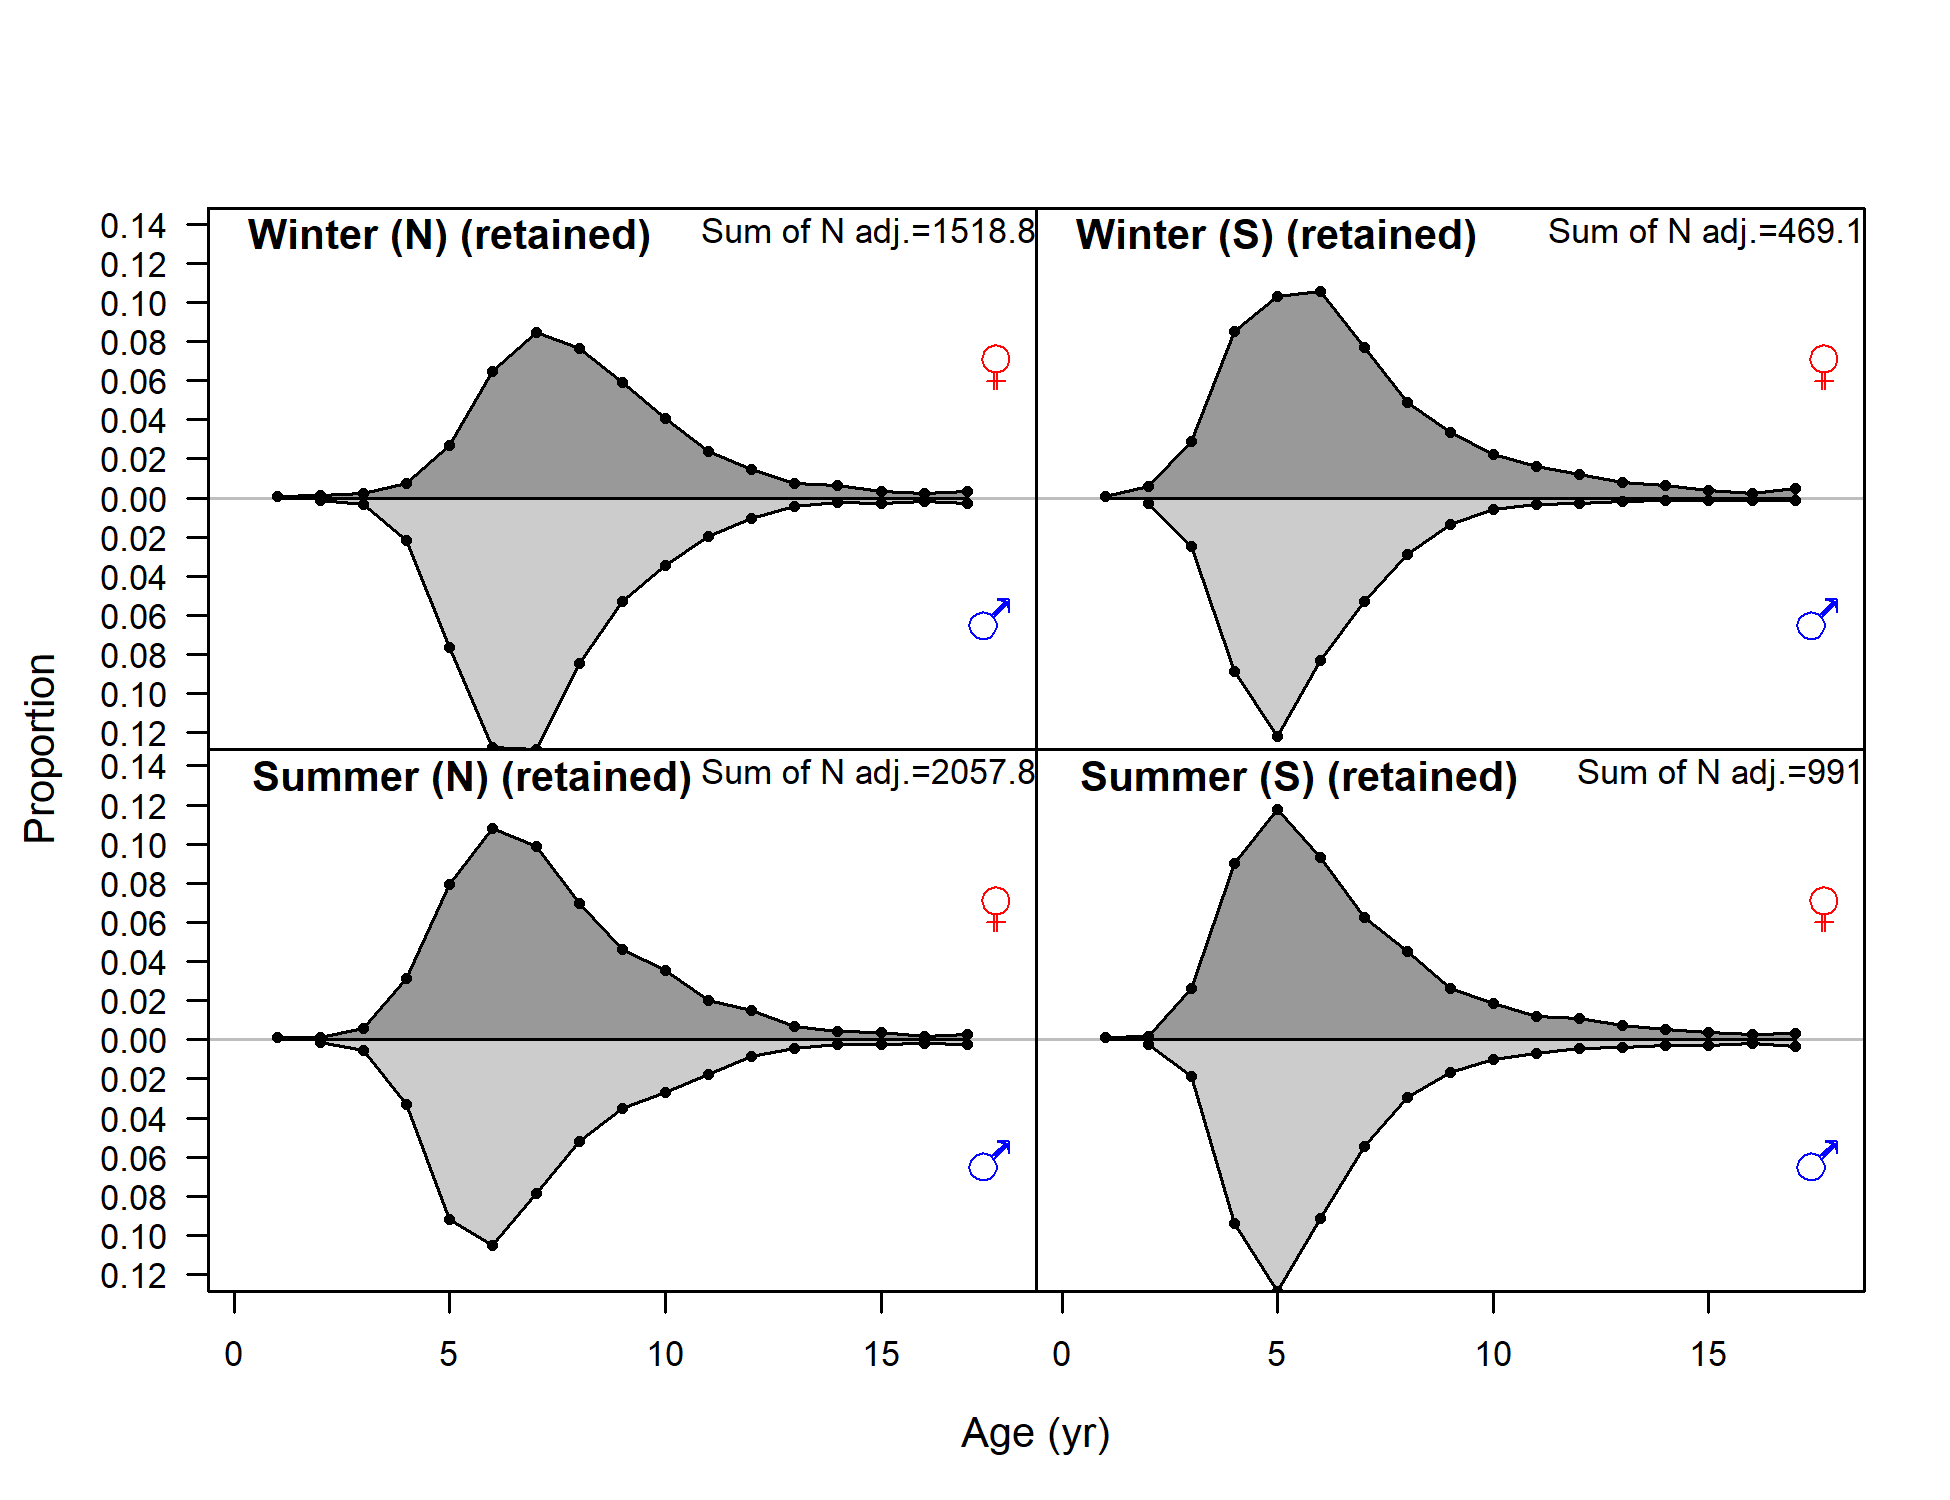
\includegraphics[scale = 0.37]{figures/comp_agedat__aggregated_across_time.png}
\end{frame}



%---------------------------------------------------------------------------
\section*{Appendix}
%----------------------------------------------------------------------------
\begin{frame}
  \Huge{\centerline{Additional data slides}}
\end{frame}

  
\end{document}
